% optimized scan design

%%%%%%%%%%%%%%%%%%%%%%%%%%%%%%%%%%%%%%%%%%%%%%%%%%%
\section{Introduction}
\label{s,scn-dsgn,intro}
%%%%%%%%%%%%%%%%%%%%%%%%%%%%%%%%%%%%%%%%%%%%%%%%%%%

Fast, accurate \emph{relaxometry}, 
or quantification
of spin-lattice and spin-spin relaxation parameters $\To$ and $\Tt$ 
has been of longstanding interest in MRI. 
Many researchers have suggested 
that $\To, \Tt$ ``maps''
(\ie, estimated parameter images)
may serve as biomarkers 
for monitoring the progression 
of various disorders \cite{cheng:12:pma}. 
Neurological applications include: 
lesion classification in multiple sclerosis 
\cite{larsson:88:ivd}; 
tumor characterization 
\cite{kurki:96:tco, englund:86:rti}; 
and symptom onset prediction in stroke 
\cite{siemonsen:09:qtv, dewitt:87:nnc}. 
In addition, 
$\To, \Tt$ have shown promise 
for detecting hip and knee cartilage degeneration 
\cite{matzat:13:qmt, mosher:04:cmt} 
and for assessing cardiac dysfunction 
due to iron overload \cite{guo:09:mtq} 
or edema \cite{giri:09:tqf}. 
Motivated by this broad interest 
in $\To, \Tt$ mapping, 
this chapter describes a systematic method 
to guide QMRI scan design.

Classical pulse sequences 
such as inversion/saturation recovery (IR/SR) 
or (single) spin echo (SE) 
yield relatively simple methods 
for $\To$ or $\Tt$ estimation, respectively; 
however, these methods require several scans, 
each with long repetition time $\TR$, 
leading to undesirably long acquisitions. 
Numerous modifications 
such as the Look-Locker method \cite{look:70:tsi}, 
multi-SE trains \cite{carr:54:eod}, 
or fast $\mathbf{k}$-space trajectories 
\cite{stehling:91:epi, ahn:86:hss, meyer:92:fsc} 
have been proposed to accelerate $\To$ 
\cite{kay:91:pia, gowland:92:faa, messroghli:04:mll, stehling:90:ire} 
and $\Tt$ 
\cite{bonny:96:tml, kumar:12:bau, beneliezer:15:raa, nguyen:12:ttd} 
relaxometry 
with these classical sequences.
These techniques are more sensitive 
to model non-idealities 
\cite{majumdar:86:eit-1, majumdar:86:eit-2, farzaneh:90:aot}, 
and are still speed-limited 
by the long $\TR$ required 
for (near)-complete $\To$ recovery.

Steady-state (SS) pulse sequences 
\cite{hinshaw:76:ifb, scheffler:99:apd} 
permit short $\TR$, 
and are thus inherently much faster 
than classical counterparts.
SS techniques are well-suited for relaxometry 
because the signals produced are highly sensitive 
to $\To$ and $\Tt$ variation. 
However, short $\TR$ times also cause SS signals 
to be complex functions 
of both desired and undesired (\emph{nuisance}) parameters, 
complicating quantification. 
Furthermore, some such methods 
\cite{deoni:03:rct, chang:08:lls} 
still require scan repetition, 
though individual scans are now considerably shorter. 
Despite these difficulties, 
the potential for rapid scanning 
with high $\To, \Tt$ sensitivity 
has motivated numerous SS relaxometry studies 
\cite{fram:87:rco, deoni:03:rct, chang:08:lls, wang:12:srt, deoni:04:rte, deoni:09:trt, welsch:09:reo, heule:14:reo, stocker:14:mpq, heule:14:tes-mrm}.

The dual-echo steady-state (DESS) sequence \cite{bruder:88:ans} 
was recently proposed as a promising SS imaging technique 
for $\Tt$ estimation \cite{welsch:09:reo}. 
Because it produces two distinct signals per excitation, 
the DESS sequence can reduce scan repetition requirements 
by recording twice as much data per scan. 
As with other SS methods, 
the resulting signals 
\cite{gyngell:89:tss, hanicke:03:aas} 
are complicated functions 
of $\To$, $\Tt$, and other parameters
(see Section~\ref{sss,bkgrd,mri,ss,dess}
for derivations). 
Prior works have isolated $\Tt$ dependencies 
using either algebraic manipulations 
of the first- and second-echo signals 
\cite{welsch:09:reo, heule:14:reo} 
or separate scans to first estimate nuisance parameters 
\cite{nataraj:14:mbe}. 
Although DESS concurrently encodes rich $\To$ and $\Tt$ information, 
these methods have shied away from using DESS 
for $\To$ estimation, 
either through bias-inducing approximations, 
or noise-propagating sequential estimation, 
respectively. 

Whether it be with DESS, other sequences, or even combinations thereof, 
it is generally unclear how to best assemble a \emph{scan profile} 
(\emph{i.e.}, a collection of scans) 
for a fixed amount of scan time. 
Furthermore, for a given scan profile, 
it is typically not obvious how 
to best select acquisition parameters 
(\emph{e.g.}, flip angles, repetition times, etc.) 
for relaxometry. 
In this and subsequent chapters, 
the term \emph{scan design} refers 
to the related problems 
of scan profile selection 
and acquisition parameter optimization.

Historically, scan design for relaxometry
has mainly been explored 
using figures of merit related to estimator precision. 
In particular, several studies have used the \Cramer-Rao Bound (CRB), 
a statistical tool that bounds the minimum variance of an unbiased estimator.
Earlier works have used the CRB and variations 
to select inversion times for recovery experiments 
\cite{weiss:80:tco, zhang:98:dos}, 
flip angles for spoiled gradient-recalled echo (SPGR) sequences \cite{wang:87:otp}, 
and echo times for SE experiments \cite{jones:96:oss}. 
More recent studies have considered additional scan design challenges, 
including scan time constraints \cite{imran:99:tpm}, 
multiple latent parameters \cite{deoni:04:doo}, 
multiple scan parameter types \cite{fleysher:07:otp}, 
and latent parameter spatial variation \cite{akcakaya:15:ots, lewis:16:ddo}. 

The aforementioned studies consider scan parameter optimization 
for profiles consisting of \emph{only one} pulse sequence.
In contrast, this chapter introduces a general framework 
for robust, application-specific scan design 
for parameter estimation from \emph{combinations} of pulse sequences.
The framework first finds multiple sets of scan parameters 
that achieve precise estimation 
within a tight, \emph{application-specific} range 
of object parameters (\emph{e.g.}, $\To, \Tt$, etc.).
The framework then chooses the one scan parameter set 
most \emph{robust} to estimator precision degradation 
over a broader range of object parameters.
As a detailed example, 
we optimize three combinations of SPGR and DESS sequences 
for $\To, \Tt$ mapping. 
For a fixed total scan time, 
we find that well-chosen DESS scans alone 
can be used to estimate both $\To$ and $\Tt$ 
with precision and robustness comparable 
to combinations of SPGR and DESS. 
This example illustrates that, 
with careful scan profile design, 
well-established pulse sequences 
can find use in new estimation problems.

This chapter is organized as follows. 
Section~\ref{s,scn-dsgn,crb} describes 
a CRB-inspired min-max optimization problem 
for robust, application-specific scan optimization. 
Section~\ref{s,scn-dsgn,opt} optimizes 
three practical DESS/SPGR combinations 
to show that, 
even in the presence of radiofrequency (RF) field inhomogeneity, 
DESS is a promising option for $\To, \Tt$ relaxometry.  
Section~\ref{s,scn-dsgn,exp} describes 
simulation, phantom, and \invivo experiments 
and discusses corresponding results.
Section~\ref{s,scn-dsgn,disc} discusses practical challenges 
and suggests future directions.
Section~\ref{s,scn-dsgn,conc} summarizes key contributions.

%%%%%%%%%%%%%%%%%%%%%%%%%%%%%%%%%%%%%%%%%%%%%%%%%%%
\section{A CRB-Inspired Scan Selection Method}
\label{s,scn-dsgn,crb}
%%%%%%%%%%%%%%%%%%%%%%%%%%%%%%%%%%%%%%%%%%%%%%%%%%%

%%%%%%%%%%%%%%%%%%%%%%%%%%%%%%%%%%%%%%%%%%%%%%%%%%%
\subsection{The CRB and its Relevance to QMRI}
\label{ss,scn-dsgn,crb,sig}

Recall from Section~\ref{ss,relax,meth,prof}
that after image reconstruction,
vwe can model the single-voxel MR image domain data
associated with a particular scan profile as 
\begin{align}
	\bmy = \bms\paren{\bmx; \bmnu, \bmP} + \bmeps,
	\label{eq:scn-dsgn,mod-vec-abbrev}
\end{align}
where signal model
$\bms := \brac{s_1, \dots, s_D}\tpose
: \complexes{L} \times \complexes{K} \times \reals{A \times D} \mapsto \complexes{D}$
relates latent $\bmx \in \complexes{L}$,
known $\bmnu \in \complexes{K}$,
and acquisition $\bmP \in \reals{A \times D}$ parameters
to noisy scan profile image data $\bmy \in \complexes{D}$, 
barring noise $\bmeps \in \complexes{D}$.
Assuming (as in Section~\ref{ss,relax,meth,prof})
complex Gaussian noise $\bmeps \sim \cgauss{\mathbf{0}}{\bmSig}$,
the likelihood function \eqref{eq:relax,lf-vec} is
(to within constants independent of $\bmx$)
\begin{align}
	\Lf{\bmx|\bmy} \propto
		\expa{-\norm{\bmy - \bms\paren{\bmx; \bmnu, \bmP}}^2_{\bmSig^{-1}}}.
	\label{eq:scn-dsgn,lf-vec}
\end{align}
Under suitable regularity conditions
\footnote{In particular,
$\bms$ must be analytic in complex components
of $\bmx$.},
the Fisher information matrix 
$\Fisher{\bmx; \bmnu, \bmP} \in \complexes{L \times L}$
\cite{fisher:1925:tos}
characterizes the imprecision 
of unbiased estimates 
of $\bmx$ from $\bmy$, 
given $\bmnu$ and $\bmP$:
\begin{align}
	\Fisher{\bmx; \bmnu, \bmP} 
		&:= 
		\expect{\bmy}{\paren{\grada{\bmx} \log{\Lf{\bmx|\bmy}}}\ctpose
		\grada{\bmx} \log{\Lf{\bmx|\bmy}}} 
		\nonumber \\
		&= 
		\paren{\grada{\bmx} \bms\paren{\bmx; \bmnu, \bmP}}\ctpose
		\bmSig^{-1} \grada{\bmx} \bms\paren{\bmx; \bmnu, \bmP}
		\label{eq:scn-dsgn,fisher},
\end{align}
where $\expect{\bmy}{\cdot}$ denotes element-wise expectation
with respect to $\bmy$.
In particular,
the matrix CRB \cite{cramer:46} ensures
that any unbiased estimator $\est{\bmx}$ satisfies
\begin{align}
	\cov{\est{\bmx}; \bmnu, \bmP} \succeq
		\bmF^{-1}\paren{\bmx; \bmnu, \bmP},
		\label{eq:scn-dsgn,crb}
\end{align}
where for arbitrary, equally-sized $\Const{1}$ and $\Const{2}$,
matrix inequality $\Const{1} \succeq \Const{2}$ 
means $\Const{1}-\Const{2}$ is positive semi-definite.
In the following,
we design an optimization problem 
based on the CRB
to guide QMRI scan design 
for relaxometry.

%%%%%%%%%%%%%%%%%%%%%%%%%%%%%%%%%%%%%%%%%%%%%%%%%%%
\subsection{Min-max Optimization Problem for Scan Design}
\label{ss,scn-dsgn,crb,minmax}

Following \cite{chernoff:53:lod}, 
we focus on minimizing a weighted average 
of the variances 
in each of the $L$ latent object parameter estimates. 
A reasonable objective function 
for overall estimator precision 
is therefore given by
\begin{align}
	\costa{\bmx; \bmnu, \bmP} =
		\trace{\bmW \bmF^{-1}\paren{\bmx; \bmnu, \bmP} \bmW\tpose}, 
		\label{eq:scn-dsgn,cost}
\end{align}
where $\bmW \in \reals{L \times L}$ 
is a diagonal, application-specific  matrix of weights, 
preselected to control the relative importance 
of precisely estimating the $L$ latent object parameters. 
For scan design, 
we would like to minimize \eqref{eq:scn-dsgn,cost} 
with respect to scan parameters $\bmP$.
 
The CRB depends not only on $\bmP$ 
but also on the spatially varying object parameters 
$\bmx$ and $\bmnu$. 
Thus, one cannot perform scan design 
by ``simply'' minimizing $\cost$ 
with respect to scan parameters $\bmP$. 
Instead, we pose a 
\emph{min-max} optimization problem 
for scan design: 
we seek candidate scan parameters $\bmPc$ 
over a search space $\setP$ 
that \emph{minimize} the worst-case 
(\emph{i.e.}, \emph{maximum}) 
cost $\costwt$, 
as viewed over ``tight'' object parameter ranges 
$\setXt$ and $\setNt$:
\begin{align}
	\breve{\bmP} &\in 
		\set{\argmin{\bmP \in \setP} \costawt{\bmP}}, \where 
		\label{eq:scn-dsgn,P-cand} \\
	\costawt{\bmP} &:=
		\max_{\substack{\bmx \in \setXt \\ \bmnu \in \setNt}}
		\costa{\bmx; \bmnu, \bmP}.
		\label{eq:scn-dsgn,cost-tight}
\end{align}
Here, 
we select \emph{latent} parameter set $\setXt$ 
based on the application 
and \emph{known} parameter set $\setNt$ 
based on the spatial variation typically observed 
in the known parameters $\bmnu$. 
Min-max approach \eqref{eq:scn-dsgn,P-star} 
should ensure good estimation precision 
over a range of parameter values.

Since $\Psi$ is in general non-convex 
with respect to $\bmP$, 
it may have multiple global minimizers 
as well as other scan parameters 
that are nearly global minimizers. 
To improve robustness 
to object parameter variations, 
we form an expanded set of candidate scan parameters 
by also including scan parameters 
that yield costs to within a tolerance $\delta \ll 1$ 
of the optimum. 
Mathematically, 
we define this expanded set 
of candidate scan parameter combinations 
(for a given scan profile) as 
\begin{align}
	\setPc &:= 
		\set{\bmP : \costawt{\bmP} - \costawt{\bmPc} \le \delta \costawt{\bmPc}}.
		\label{eq:scn-dsgn,set}
\end{align}
To select amongst these candidate scan parameters, 
we employ a robustness criterion: 
we select the single scan parameter $\bmPs$ 
that degrades the least 
when the worst-case cost is viewed 
over widened object parameter sets 
$\setXb \supseteq \setXt$ and $\setNb \supseteq \setNt$:
\begin{align}
	\bmPs &= 
		\argmin{\bmP \in \setPc} \costawb{\bmP}, \where
		\label{eq:scn-dsgn,P-star} \\
	\costawb{\bmP} &:=
		\max_{\substack{\bmx \in \setXb \\ \bmnu \in \setNb}}
		\costa{\bmx; \bmnu, \bmP}.
		\label{eq:scn-dsgn,cost-broad}
\end{align}
To compare different scan profiles, 
we select corresponding search spaces $\setP$ 
to satisfy acquisition constraints 
(\emph{e.g.}, total scan time), 
but otherwise hold optimization parameters 
$\bmW$, $\delta$, $\setXt$, $\setXb$, $\setNt$, $\setNb$ fixed.
Since $\Psi$ is data-independent, 
we can solve \eqref{eq:scn-dsgn,P-cand} and \eqref{eq:scn-dsgn,P-star} offline 
for each scan profile. 
The result of each profile's min-max optimization process \eqref{eq:scn-dsgn,P-star} 
is a corresponding optimized scan parameter matrix $\bmPs$ 
that is suitable for the range 
of latent $\bmx$ and known $\bmnu$ object parameters specified 
in $\setXt$ and $\setNt$, 
and is robust to variations in those parameters 
over broader sets $\setXb$ and $\setNb$, 
respectively.

%%%%%%%%%%%%%%%%%%%%%%%%%%%%%%%%%%%%%%%%%%%%%%%%%%%
\section{Optimizing SS Sequences for Relaxometry in the Brain}
\label{s,scn-dsgn,opt}
%%%%%%%%%%%%%%%%%%%%%%%%%%%%%%%%%%%%%%%%%%%%%%%%%%%

This section applies the methods 
of Section~\ref{ss,scn-dsgn,crb,minmax} 
to the problem of scan design 
for joint $\To,\Tt$ estimation 
from combinations of SS sequences. 
Section~\ref{ss,scn-dsgn,opt,design} details 
how we use optimization problems
\eqref{eq:scn-dsgn,P-cand} and \eqref{eq:scn-dsgn,P-star} 
to tailor three SPGR and DESS scan combinations
for precise $\To,\Tt$ estimation 
in white matter (WM) and grey matter (GM) regions 
of the brain. 
Section~\ref{ss,scn-dsgn,opt,compare} compares the predicted performance 
of the three optimized scan profiles.

%%%%%%%%%%%%%%%%%%%%%%%%%%%%%%%%%%%%%%%%%%%%%%%%%%%
\subsection{Scan Design Details}
\label{ss,scn-dsgn,opt,design}

There are numerous candidate scan profiles
involving DESS and/or other pulse sequences
that may be useful
for fast, accurate $\To,\Tt$ mapping.
In this chapter,
we consider combinations
of magnitude SPGR and DESS scans
for estimating the $L\gets3$ latent parameters
$\To,\Tt$, and proportionality constant $\const{2}$
(defined in Example~\ref{sss,relax,meth,sig,t2}),
given knowledge 
of transmit field inhomogeneity $\stx$
as $K \gets 1$ known parameter.
With proper RF phase cycling
and gradient spoiling,
the SPGR signal $\spgr$
(as expressed in \eqref{eq:spgr-model})
contains no explicit $\Tt$ dependence.
SPGR's reduced dependence
on spatially varying unknowns
is reason for its use in $\To$ mapping
\cite{fram:87:rco, chang:08:lls, wang:12:srt}
and subsequent $\Tt$ mapping
from other sequences
\cite{deoni:03:rct, nataraj:14:mbe}.
In a similar spirit, 
we examine scan profiles containing SPGR 
over other SS sequences because we predict 
that the SPGR sequence's $\Tt$-independence 
may help estimators disentangle $\Tt$ 
from other unknown sources of DESS signal contrast.

As respectively discussed
in Examples~\ref{sss,relax,meth,sig,t1}-\ref{sss,relax,meth,sig,t2},
each SPGR and DESS scan leaves 
$\bmp \gets [\flipnom, \TR]\tpose$
as $A \gets 2$ acquisition parameters
available to optimize.
A given scan profile consisting 
of $\Ss$ SPGR and $\Sd$ DESS scans 
yields $D \gets \Ss + 2\Sd$ datasets. 
We optimize such a scan profile 
by solving \eqref{eq:scn-dsgn,P-star} 
over a dimension-$AD \gets 2(\Ss + 2\Sd)$ space 
of scan parameters.

We select constraints 
on search space $\setP$ based 
on hardware limitations 
and desired scan profile properties. 
Since each pair of DESS signals 
must share the same $\bmp$, 
the search space $\setP$ is reduced to 
$\setAs^{\Ss} \times \setAd^{\Sd} \times \setTRs^{\Ss} \times \setTRd^{\Sd}$ 
(superscripts denote Cartesian powers). 
We assign flip angle ranges 
$\setAs \gets \brac{5, 90}^\circ$ 
and $\setAd \gets \brac{5, 90}^\circ$
to restrict RF energy deposition. 
We set feasible $\TR$ solution sets 
$\setTRs \gets [12.2, +\infty)$ms 
and $\setTRd \gets [17.5, +\infty)$ms 
based on pulse sequence designs 
that control for other scan parameters. 
These control parameters are described 
in further detail in Section~\ref{s,scn-dsgn,exp}, 
and are held fixed 
in all subsequent SPGR and DESS experiments. 
To equitably compare optima 
from different scan profiles, 
we require 
$$\bmTR := [T_{\mathrm{R},1}, \dots, T_{\mathrm{R},{\Ss}}, 
T_{\mathrm{R},{\Ss}+1}, \dots, T_{\mathrm{R},{\Ss + \Sd}}]\tpose$$ 
to satisfy a total time constraint, 
$\norm{\bmTR}_1 \le \Tmax$. 
For a scan profile consisting 
of $\Ss$ SPGR and $\Sd$ DESS scans, 
these constraints collectively reduce the search space dimension 
from $AD$ to $2(\Ss + \Sd) -1$. 

Prior works have considered $\To$ or $\Tt$ estimation 
from as few as 2 SPGR 
\cite{wang:87:otp, deoni:03:rct} 
or 1 DESS \cite{welsch:09:reo} scan(s), 
respectively. 
We likewise elect to optimize 
the $(\Ss, \Sd) \gets (2,1)$ scan profile 
as a benchmark. 
We choose $\Tmax \gets 2(12.2) + 1(17.5) = 41.9$ms 
and select other scan profiles capable 
of meeting this time constraint. 
Requiring that candidate profiles contain $\Sd \ge 1$ DESS scans 
for $\Tt$ contrast and satisfy $D \ge L (=3)$ 
for well-conditioned estimation, 
we note that $(1,1)$ and $(0,2)$ 
are the only other eligible profiles. 

In the ensuing experiments, 
we focus on precise $\To,\Tt$ estimation in the brain.
Noting that $\To\sim10\Tt$, 
we choose $\mathbf{W} \gets \mathrm{diag}\paren{0.1, 1, 0}$ 
to place approximately equal importance 
on precise $\To$ versus $\Tt$ estimation
and zero weight
on proportionality constant $\const{2}$ estimation
(obviating the need
for complex differentiation
in \eqref{eq:scn-dsgn,fisher}).
Since $\cost$ then depends 
on $\const{2}$ through only a scale factor,
it suffices to fix $\const{2} \gets 1$
and design the latent object parameter range
as $\setXt \gets \setTot \times \setTtt \times 1$.
Here, 
$\setTot \gets [800, 1400]$ms
and $\setTtt \gets [50, 120]$ms
correspond with WM and GM regions of interest (ROIs)
at 3T \cite{wansapura:99:nrt, stanisz:05:ttr}.
We take $\setNt \gets \brac{0.9, 1.1}$ 
to account for 10\% transmit field spatial variation. 
Broadened ranges 
$\setXb \gets [400, 2000]\text{ms} \times [40, 200]\text{ms} \times 1$ 
and $\setNb \gets [0.5, 2]$ are constructed 
to encourage solutions robust 
to a realistically wide range of object parameters. 
We assume constant noise variance 
$\sigma_1^2 = \dots = \sigma_D^2 := \sigma^2$, 
where $\sigma^2 \gets 1.49 \times 10^{-7}$ is selected 
to reflect measurements from normalized phantom datasets 
(\emph{cf.} Section~\ref{sss,scn-dsgn,exp,phant,roi}  
for acquisition details).
Lastly, we set $\delta \gets 0.01$ 
to select a robust scan parameter $\bmPs$ 
with associated worst-case cost $\costawt{\bmPs}$ 
within 1\% of global optimum $\costawt{\bmPc}$.

%%%%%%%%%%%%%%%%%%%%%%%%%%%%%%%%%%%%%%%%%%%%%%%%%%%
\subsection{Scan Profile Comparisons}
\label{ss,scn-dsgn,opt,compare} 

We solve \eqref{eq:scn-dsgn,P-cand} and \eqref{eq:scn-dsgn,P-star} 
via grid search 
to allow illustration 
of $\costwt(\bmP)$ 
as well as worst-case $\To,\Tt$ standard deviations 
$\sigwot(\bmP)$ and $\sigwtt(\bmP)$, 
each defined as
\begin{align}
	\sigwot(\bmP) &:= 
		\max_{\substack{\bmx \in \setXt \\ \bmnu \in \setNt}} 
		\sigma_{\To}(\bmx; \bmnu, \bmP); 
		\label{eq:scn-dsgn,sigwot} \\
	\sigwtt(\bmP) &:= 
		\max_{\substack{\bmx \in \setXt \\ \bmnu \in \setNt}} 
		\sigma_{\Tt}(\bmx; \bmnu, \bmP), 
		\label{eq:scn-dsgn,sigwtt} 
\end{align}
where $\sigma_{\To}(\bmx; \bmnu, \bmP)$ 
and $\sigma_{\Tt}(\bmx; \bmnu, \bmP)$ 
are corresponding diagonal elements 
of inverse Fisher matrix $\bmF^{-1}(\bmx; \bmnu, \bmP)$. 
Grid searches for the $(2,1)$, $(1,1)$, and $(0,2)$ profiles 
each took about 4, 43, and 28 minutes, respectively.
All experiments described hereafter were carried out 
using MATLAB\regis R2013a 
on a 3.5GHz desktop with 32GB RAM. 

\begin{table*} [!tb]
	\centering
	{\tabulinesep = 0.5mm
	\begin{tabu} {r | c c c}
		\hline \hline 
		Scan & $(2,1)$ & $(1,1)$ & $(0,2)$ \\
		\hline
		$\widehat{\alpha}^{\mathrm{spgr}}_0$ & (15,5)$^\circ$ & 15$^\circ$ & -- \\
		$\widehat{\alpha}^{\mathrm{dess}}_0$ & 30$^\circ$ & 10$^\circ$ & (35,10)$^\circ$ \\
		$\widehat{T}_{R}^\mathrm{spgr}$ & (12.2, 12.2) & 13.9 & -- \\
		$\widehat{T}_{R}^\mathrm{dess}$ & 17.5 & 28.0 & (24.4, 17.5) \\
		\hline
		$\sigwot(\bmPs)$ & 28 & 27 & \textbf{21} \\
		$\sigwob(\bmPs)$ & 154 & 169 & \textbf{113} \\
		\hline
		$\sigwtt(\bmPs)$ & \textbf{1.3} & 2.8 & 1.5 \\
		$\sigwtb(\bmPs)$ & 9.1 & 8.8 & \textbf{6.0} \\
		\hline
		$\costwt(\bmPs)$ & 4.0 & 4.9 & \textbf{3.5} \\
		$\costwb(\bmPs)$ & 17.7 & 17.9 & \textbf{12.2} \\
		\hline \hline
	\end{tabu}}
	\vspace{1mm}
	\caption{Performance summary of different scan profiles, 
		optimized by solving \eqref{eq:scn-dsgn,P-star} subject 
		to scan time constraint $\Tmax = 41.9$ms. 
		The first row defines each profile. 
		The next four rows describe $\bmPs$. 
		The latter three pairs of rows 
		show how worst-case values degrade 
		from tight to broad ranges. 
		Flip angles are in degrees; 
		all other values are in milliseconds.
	}
	\label{table:profile}
\end{table*}

Table~\ref{table:profile} compares optimized scan parameters 
for profiles consisting 
of $(2,1)$, $(1,1)$, and $(0,2)$ SPGR and DESS scans, 
respectively. 
In addition to $\sigwot(\bmPs)$ and $\sigwtt(\bmPs)$, 
Table~\ref{table:profile} presents 
analogous worst-case standard deviations 
$\sigwob(\bmPs)$ and $\sigwtb(\bmPs)$ 
over $\setXb \times \setNb$ 
to show how each estimator degrades 
over the broadened object parameter range. 
When viewed over tight range 
$\setXt \times \setNt$, 
the $(0,2)$ profile provides a 11.5\% reduction 
in worst-case cost over the other choices. 
Extending to broadened range $\setXb \times \setNb$, 
this reduction grows dramatically to 31.4\%. 
We thus observe that while the different optimized profiles 
afford similar estimator precision 
over a narrow range of interest, 
the $(0,2)$ profile may be preferable 
due to its robustness to a wide range of object parameters. 

\begin{sidewaysfigure} [!tbp]
	\centering
	\fbox{ 
		\begin {minipage} [b] [12.5cm] [b] {0.54\textwidth}
			\subfigure [$\sigwot$ vs. $(\alpha_1^\mathrm{spgr}, \alpha_2^\mathrm{spgr})$] {
				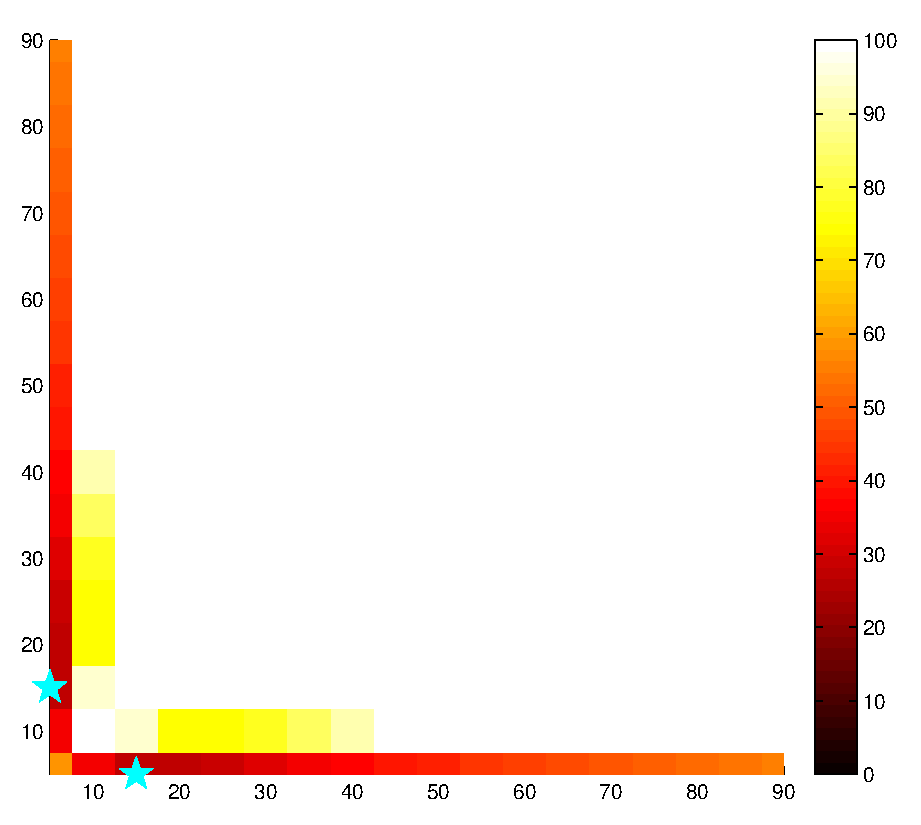
\includegraphics [height=3.41cm] {sigw_t1_vs_s1s2_21_41p90ms_0p1_1.eps}
				\label{fig:sigw,t1,s1s2,21}
			}
			\subfigure [$\sigwot$ vs. $(\alpha_1^\mathrm{spgr}, \alpha^\mathrm{dess})$] {
				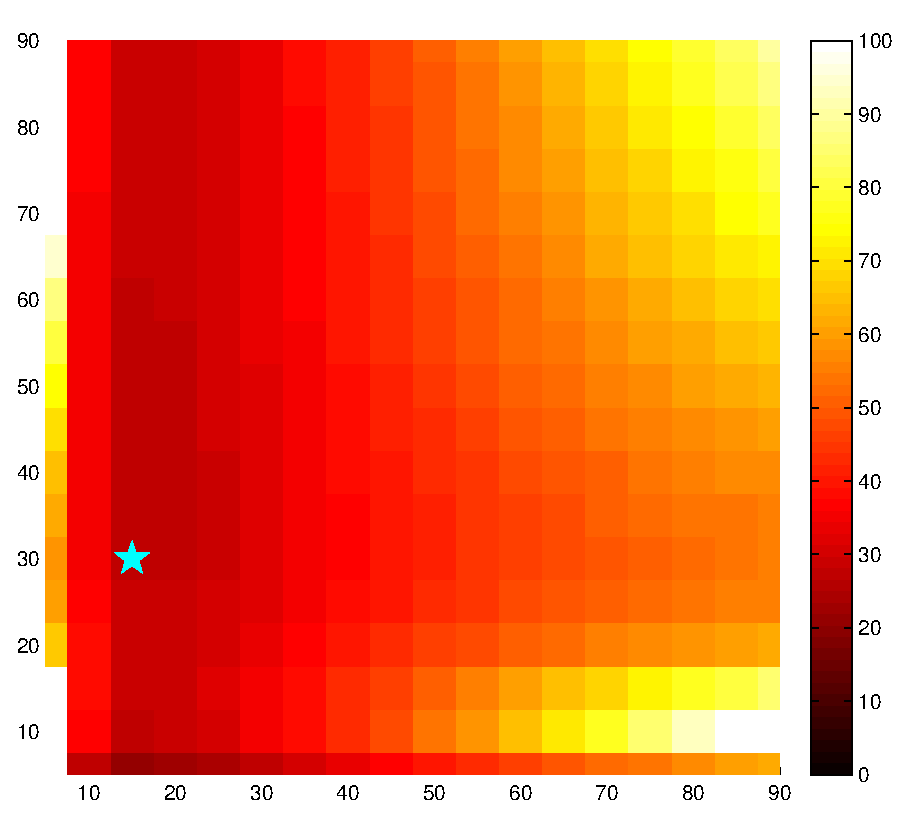
\includegraphics [height=3.41cm] {sigw_t1_vs_s1d1_21_41p90ms_0p1_1.eps}
				\label{fig:sigw,t1,s1d1,21}
			}
			\subfigure [$\sigwot$ vs. $(\alpha_2^\mathrm{spgr}, \alpha^\mathrm{dess})$] {
				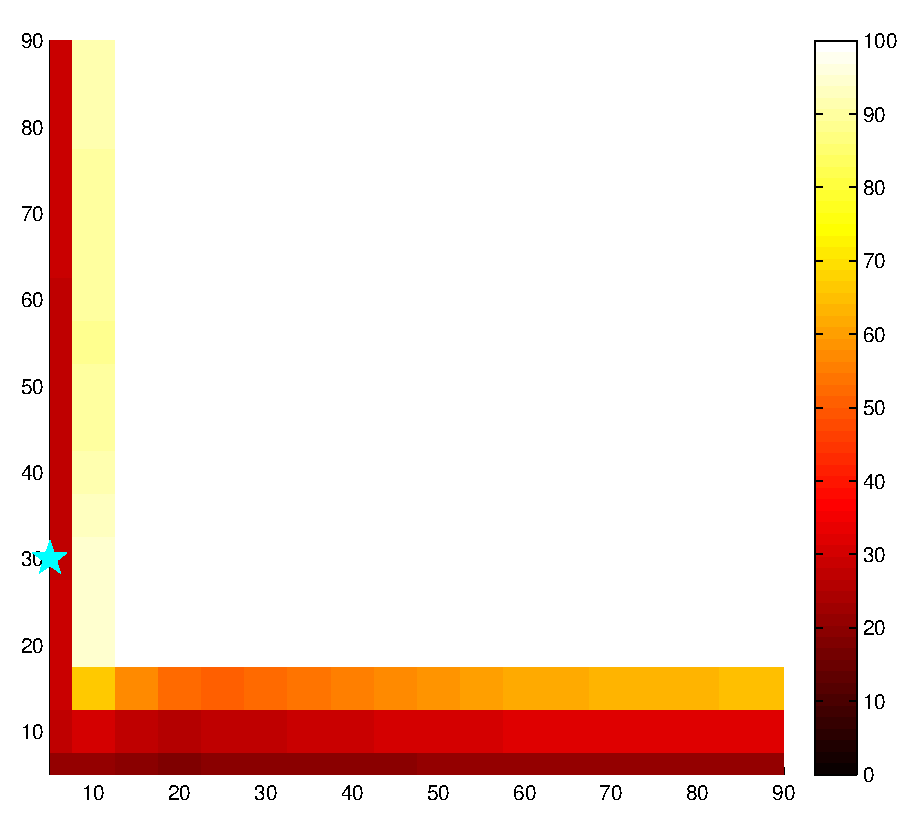
\includegraphics [height=3.41cm] {sigw_t1_vs_s2d1_21_41p90ms_0p1_1.eps}
				\label{fig:sigw,t1,s2d1,21}
			}
			
			\subfigure [$\sigwtt$ vs. $(\alpha_1^\mathrm{spgr}, \alpha_2^\mathrm{spgr})$] {
				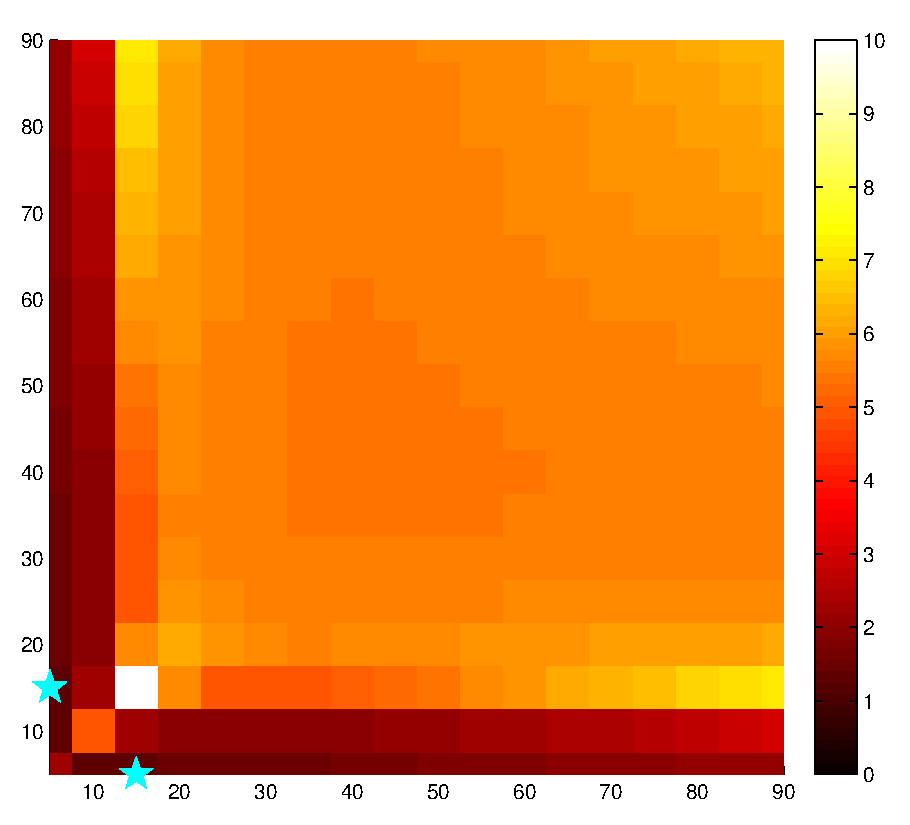
\includegraphics [height=3.41cm] {sigw_t2_vs_s1s2_21_41p90ms_0p1_1.eps}
				\label{fig:sigw,t2,s1s2,21}
			}
			\subfigure [$\sigwtt$ vs. $(\alpha_1^\mathrm{spgr}, \alpha^\mathrm{dess})$] {
				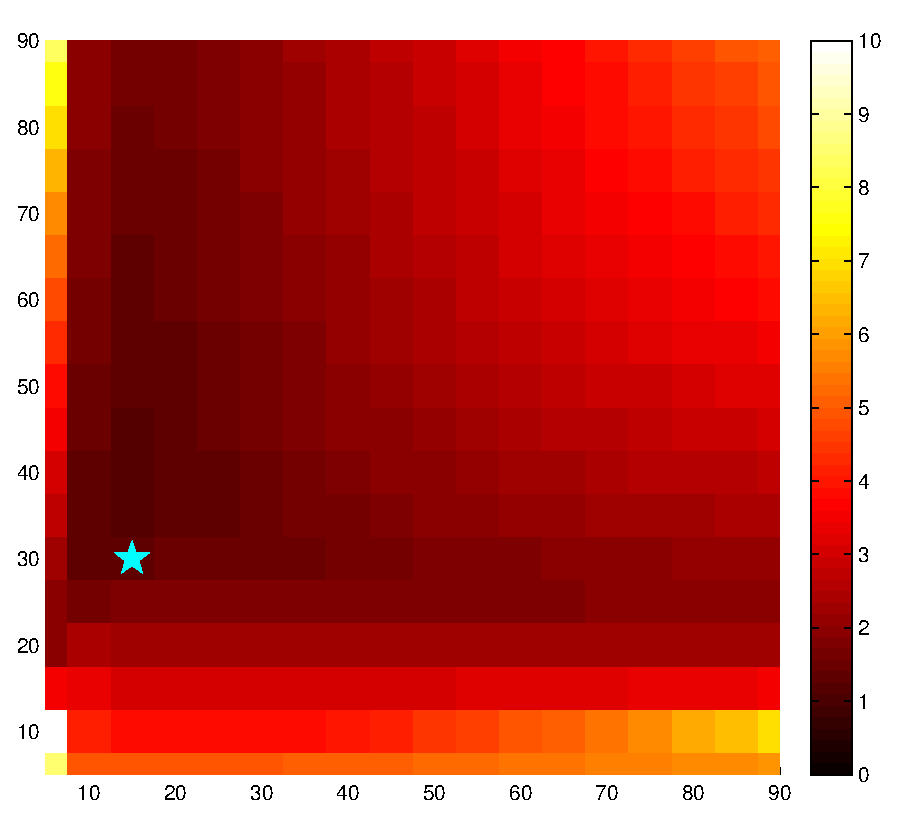
\includegraphics [height=3.41cm] {sigw_t2_vs_s1d1_21_41p90ms_0p1_1.eps}
				\label{fig:sigw,t2,s1d1,21}
			}
			\subfigure [$\sigwtt$ vs. $(\alpha_2^\mathrm{spgr}, \alpha^\mathrm{dess})$] {
				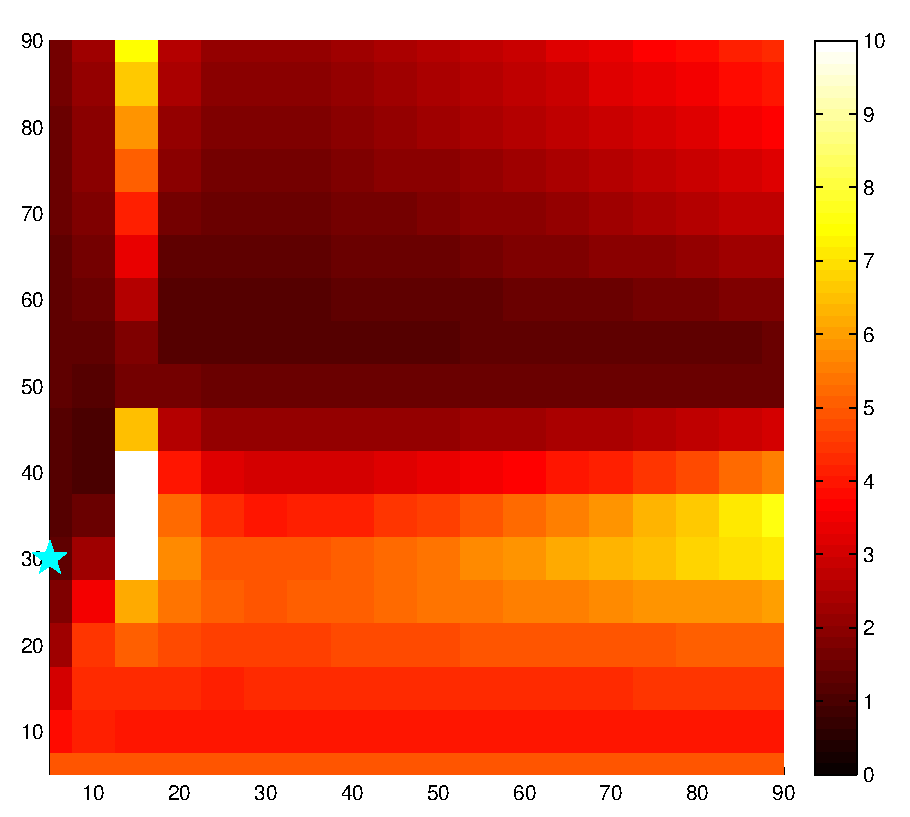
\includegraphics [height=3.41cm] {sigw_t2_vs_s2d1_21_41p90ms_0p1_1.eps}
				\label{fig:sigw,t2,s2d1,21}
			}
			
			\subfigure [$\costwt$ vs. $(\alpha_1^\mathrm{spgr}, \alpha_2^\mathrm{spgr})$] {
				\includegraphics [height=3.41cm] {Psiw_vs_s1s2_21_41p90ms_0p1_1.eps}
				\label{fig:sigw,t1,s1s2,21}
			}
			\subfigure [$\costwt$ vs. $(\alpha_1^\mathrm{spgr}, \alpha^\mathrm{dess})$] {
				\includegraphics [height=3.41cm] {Psiw_vs_s1d1_21_41p90ms_0p1_1.eps}
				\label{fig:sigw,t1,s1d1,21}
			}
			\subfigure [$\costwt$ vs. $(\alpha_2^\mathrm{spgr}, \alpha^\mathrm{dess})$] {
				\includegraphics [height=3.41cm] {Psiw_vs_s2d1_21_41p90ms_0p1_1.eps}
				\label{fig:sigw,t1,s2d1,21}
			}
		\end{minipage}
	}
	\fbox{ 
		\begin {minipage} [b] [12.5cm] [b] {0.18\textwidth}
			\subfigure [$\sigwot$ vs. $(\alpha^\mathrm{spgr}, \alpha^\mathrm{dess})$] {
				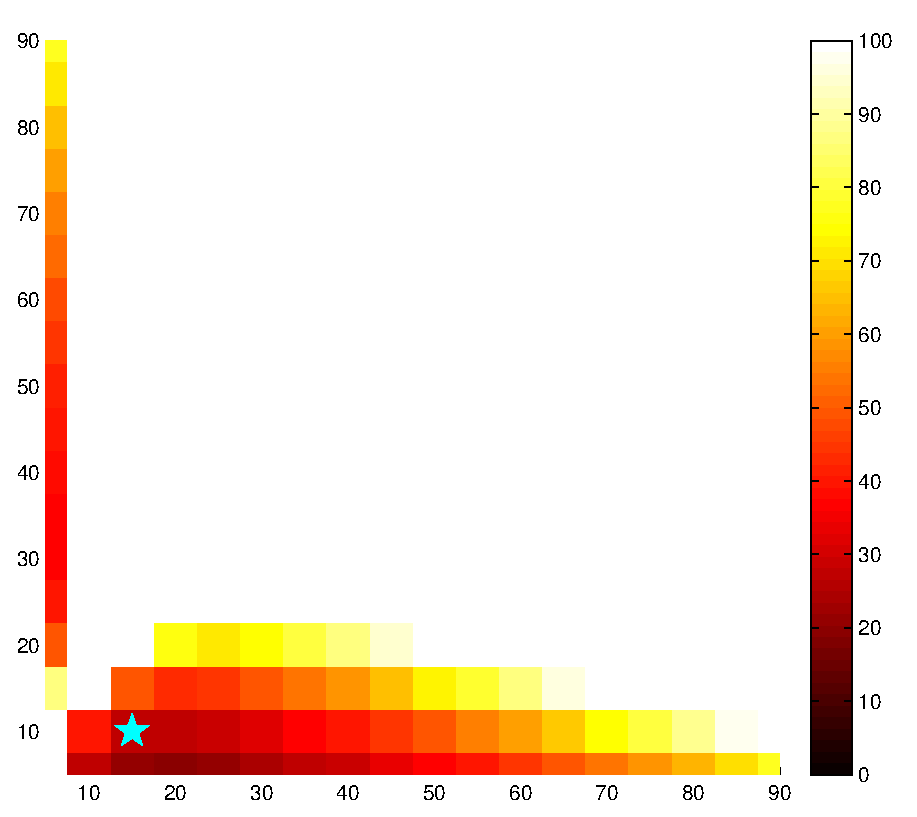
\includegraphics [height=3.41cm] {sigw_t1_vs_s1d1_11_41p90ms_0p1_1.eps}
				\label{fig:sigw,t1,s1d1,11}
			}
			
			\subfigure [$\sigwtt$ vs. $(\alpha^\mathrm{spgr}, \alpha^\mathrm{dess})$] {
				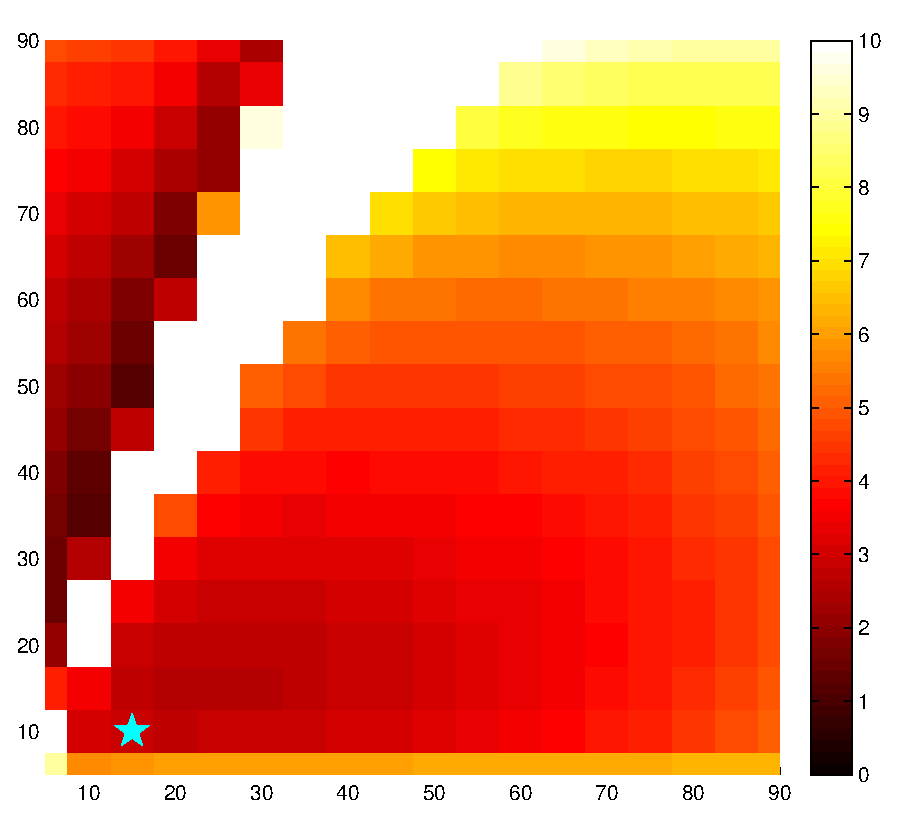
\includegraphics [height=3.41cm] {sigw_t2_vs_s1d1_11_41p90ms_0p1_1.eps}
				\label{fig:sigw,t2,s1d1,11}
			}
			
			\subfigure [$\costwt$ vs. $(\alpha^\mathrm{spgr}, \alpha^\mathrm{dess})$] {
				\includegraphics [height=3.41cm] {Psiw_vs_s1d1_11_41p90ms_0p1_1.eps}
				\label{fig:Psiw,s1d1,11}
			}
		\end{minipage}	
	}
	\fbox{ 
		\begin {minipage} [b] [12.5cm] [b] {0.18\textwidth}
			\subfigure [$\sigwot$ vs. $(\alpha_1^\mathrm{dess}, \alpha_2^\mathrm{dess})$] {
				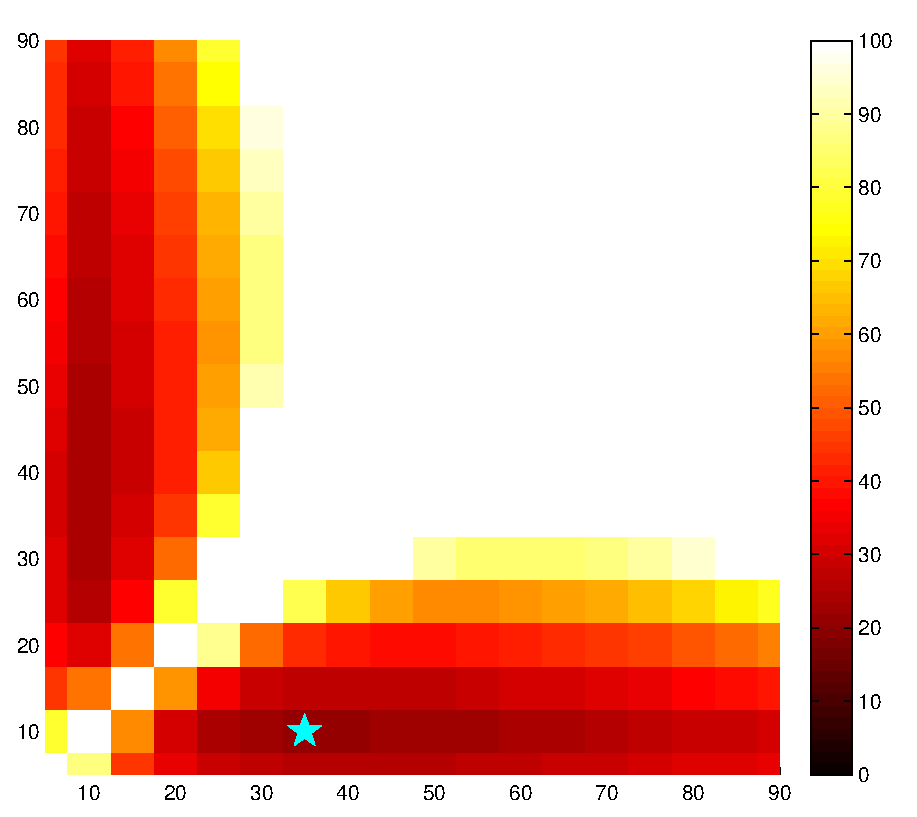
\includegraphics [height=3.41cm] {sigw_t1_vs_d1d2_02_41p90ms_0p1_1.eps}
				\label{fig:sigw,t1,d1d2,02}
			}
			
			\subfigure [$\sigwtt$ vs. $(\alpha_1^\mathrm{dess}, \alpha_2^\mathrm{dess})$] {
				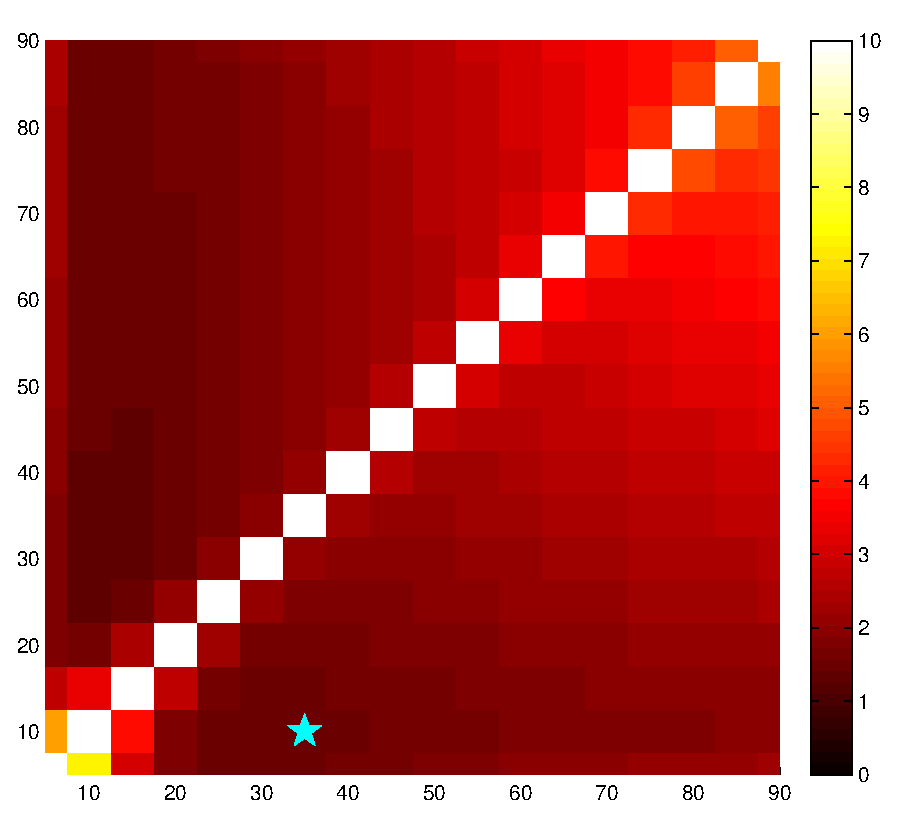
\includegraphics [height=3.41cm] {sigw_t2_vs_d1d2_02_41p90ms_0p1_1.eps}
				\label{fig:sigw,t2,d1d2,02}
			}
			
			\subfigure [$\costwt$ vs. $(\alpha_1^\mathrm{dess}, \alpha_2^\mathrm{dess})$] {
				\includegraphics [height=3.41cm] {Psiw_vs_d1d2_02_41p90ms_0p1_1.eps}
				\label{fig:Psiw,d1d2,02}
			}
		\end{minipage}	
	}
	\caption{
		Worst-case standard deviations $\sigwot$ (top), $\sigwtt$ (middle), and cost $\costwt$ (bottom), versus pairs of nominal flip angles, holding other scan parameters fixed at selected profile $\bmPs$. 
		Subfigures (a)-(i), (j)-(l), and (m)-(o) correspond to scan profiles containing $(\Ss, \Sd) = (2,1), (1,1), \text{and}\,(0,2)$ SPGR and DESS scans, respectively. 
		Selected scan parameters (starred) are within $\delta = 1$\% of global minimizers and retain as much estimator precision as possible over a wide range of latent object parameters. 		
		All axes range from 5 to 90 degrees, in 5-degree increments. 
		Colorbar ranges are $[0,100]$, $[0,10]$, and $[0,20]$ milliseconds for rows of $\sigwot$, $\sigwtt$, and $\costwt$ subfigures, respectively. 
		The optimized $(0,2)$ profile appears most robust to transmit field spatial variation.
	}
	\label{fig:heat,maps}
\end{sidewaysfigure}

Fig.~\ref{fig:heat,maps} displays heat maps 
of worst-case latent parameter standard deviations 
$\sigwot$, $\sigwtt$ 
and worst-case cost $\costwt$ 
as pairs of flip angles are varied away 
from the optimized scan design $\bmPs$.
Boxes group subfigures corresponding 
to the same scan profile. 
Viewing the bottom row of subfigures, 
it is evident 
that $\costwt(\bmPs)$ takes similar values 
for the different scan profiles. 
However, 
it is apparent that the $(\Ss,\Sd) = (0,2)$ profile 
is substantially more robust 
to transmit field variation 
than other tested profiles 
(namely, $(2,1)$ and $(1,1)$). 
Optimized worst-case cost 
over broadened latent parameter ranges 
$\costwb(\bmPs)$ captures this 
by expanding the range of possible flip angles 
from $\setNt = [0.9, 1.1]$ to $\setNb = [0.5, 2]$ 
to account for factor-of-two spatial variation 
in relative flip angle.
As a result, we find that the properties 
of ``broad'' search criterion $\costwb$ 
provide a stronger reason to select the $(0,2)$ scan 
for joint $\To, \Tt$ estimation in the brain 
than the properties 
of ``tight'' search criterion $\costwt$.

As the DESS sequence has already found success 
for $\Tt$ mapping from even one scan \cite{welsch:09:reo}, 
it is reassuring but unsurprising that our analysis finds two DESS scans 
to yield the most precise $\Tt$ estimates. 
More interestingly, 
our methods suggest that, 
with a minimum $\Sd = 2$ scans, 
DESS can be used to simultaneously estimate $\To$ as well. 
In fact, for certain choices of parameter ranges, 
a second DESS scan is predicted 
to afford $\widehat{T}_1$ precision 
comparable to two SPGR scans. 

%%%%%%%%%%%%%%%%%%%%%%%%%%%%%%%%%%%%%%%%%%%%%%%%%%%
\section{Experimental Validation and Results}
\label{s,scn-dsgn,exp}
%%%%%%%%%%%%%%%%%%%%%%%%%%%%%%%%%%%%%%%%%%%%%%%%%%%

To test our approach 
to optimized scan design 
(described in Section~\ref{ss,scn-dsgn,crb,minmax}), 
we estimate $\bmTo$ and $\bmTt$ maps 
(using maximum likelihood (ML) and 
regularized likelihood (RL) methods 
detailed in Section~\ref{ss,relax,meth,est}) 
from datasets collected 
using the scan profiles 
optimized in Section~\ref{s,scn-dsgn,opt}. 
In Section~\ref{ss,scn-dsgn,exp,sim}, 
we study estimator statistics from simulated data.
In Sections~\ref{ss,scn-dsgn,exp,phant}-\ref{ss,scn-dsgn,exp,invivo}, 
we progress to phantom and \emph{in vivo} datasets 
to evaluate scan profile performance 
under increasingly complex settings.
For the latter experiments, 
we use reference parameter maps 
from classical (long) pulse sequences, 
in lieu of ground truth maps.

%%%%%%%%%%%%%%%%%%%%%%%%%%%%%%%%%%%%%%%%%%%%%%%%%%%
\subsection{Numerical Simulations}
\label{ss,scn-dsgn,exp,sim}

We select $\To$ and $\Tt$ WM and GM values 
based on previously reported measurements 
at 3T \cite{wansapura:99:nrt, stanisz:05:ttr} 
and extrapolate other nuisance latent object parameters 
$\mzero$ and $\Tts$
from measurements at 1.5T \cite{kwan:99:msb}. 
We assign these parameter values
to the discrete anatomy 
of the BrainWeb digital phantom 
\cite{collins:98:dac, kwan:99:msb} 
to create ground truth $\bmMz, \bmTo, \bmTt, \bmTts \in \reals{V}$ maps. 
We then choose acquisition parameters based 
on Table~\ref{table:profile} 
(with fixed $\TE~=~4.67$ms) 
and apply models \eqref{eq:spgr-model} 
and \eqref{eq:dess-def-model}-\eqref{eq:dess-ref-model} 
to the 81st slices of these true maps 
to compute noiseless $217 \times 181$ SPGR and DESS image-domain data, 
respectively. 

For each scan profile, 
we corrupt the corresponding (complex) noiseless dataset $\bmS$ 
with additive complex Gaussian noise, 
whose variance $\sigma^2 \gets 1.49 \times 10^{-7}$ 
is set to match CRB calculations. 
This yields realistically noisy datasets $\bmY$ ranging 
from 105-122 signal-to-noise ratio (SNR), 
where SNR is defined here as
\begin{align}
	\snr{\bmS,\bmY} := \frac{\frob{\bmS}}{\frob{\bmY-\bmS}}.
	\label{eq:snr}
\end{align}
We use each profile's noisy magnitude dataset $\abs{\bmY}$
to compute estimates $\bmToest$ and $\bmTtest$ 
We then evaluate estimator bias and variance 
from latent ground truth $\bmTo$ and $\bmTt$ maps.

In these simulations, 
we intentionally neglect to model 
a number of physically realistic effects 
because their inclusion 
would complicate study of estimator statistics. 
First and foremost, 
we assume knowledge 
of a uniform  transmit field, 
to avoid confounding $\stx$ and $\To, \Tt$ estimation errors. 
For a similar reason, 
spatial variation in the sensitivity 
of a single receive coil is also not considered. 
We omit modeling partial volume effects 
to ensure deterministic knowledge of WM and GM ROIs. 
We will explore the influence of these (and other) nuisance effects 
on scan design in later subsections and chapters. 

To isolate bias due to estimator nonlinearity 
from regularization bias, 
we solve ML problem \eqref{eq:relax,ml-est} only,
and do not proceed to solve RL problem \eqref{eq:relax,rl-est}.
This permits consideration of $\To,\Tt$ estimation 
from each of the 7733 WM or 9384 GM data points 
as voxel-wise independent realizations 
of the same estimation problem. 
To minimize quantization bias, 
we optimize \eqref{eq:relax,ml-est} using a finely spaced dictionary 
of signal vectors from 1000 $\To$ and $\Tt$ values 
logarithmically spaced between 
$[10^2, 10^{3.5}]$ and $[10^1, 10^{2.5}]$, respectively. 
Using $10^6$ dictionary elements, 
solving \eqref{eq:relax,ml-est} took less than 7 minutes 
for each tested scan design $\bmPs$.

% T1/T2 simulation summary table
\begin{table} [!tb]
	\centering
	{\tabulinesep = 0.2mm
	\begin{tabu} {c | r r r | r}
		\hline \hline
		Scan 		& $(2,1)$ 			& $(1,1)$ 			& $(0,2)$			& Truth \\
		\hline
		WM $\ToML$	& $830 \pm 17$		& $830 \pm 15$		& $830 \pm 14$		& $832$	\\
		GM $\ToML$ 	& $1330 \pm 30.$	& $1330 \pm 24$		& $1330 \pm 24$		& $1331$ \\
		\hline
		WM $\TtML$ 	& $80. \pm 1.0$		& $80. \pm 2.1$		& $79.6 \pm 0.94$	& $79.6$ \\
		GM $\TtML$	& $110. \pm 1.4$	& $110. \pm 3.0$	& $110. \pm 1.6$ 	& $110$ \\
		\hline \hline
	\end{tabu}}
	\vspace{1mm}
	\caption{Sample means $\pm$ sample standard deviations of $\bmTo$ and $\bmTt$ ML estimates in WM and GM ROIs of simulated data, compared across different optimized scan profiles. Sample means exhibit insignificant bias, and sample standard deviations are consistent with worst-case standard deviations $\sigwot$ and $\sigwtt$ reported in Table \ref{table:profile}. All values are reported in milliseconds.}
	\label{table:numerical}
\end{table}

Table~\ref{table:numerical} verifies
\footnote{Each sample statistic presented 
in this chapter 
is rounded off to the highest place value 
of its corresponding uncertainty measure.
For simplicity, 
each uncertainty measure is itself endowed 
one extra significant figure.
Decimal points indicate the significance of trailing zeros.
}	
that, 
despite model nonlinearity and Rician noise,
estimation bias in WM- and GM-like voxels is negligible.
Sample standard deviations are consistent with $\sigwot$ and $\sigwtt$ (\emph{cf.}~Table~\ref{table:profile}). 
We observe that the $(1,1)$ and $(0,2)$ profiles afford high 
$\bmToest^\mathrm{ML}$ precision, 
while the $(2,1)$ and $(0,2)$ scans afford high 
$\bmTtest^\mathrm{ML}$ precision. 
In agreement with the predictions 
of $\costwt$ and $\costwb$, 
these simulation studies suggest that at these SNR levels,
an optimized profile containing 2 DESS scans
can permit $\bmTo$ and $\bmTt$ estimation precision 
in WM and GM comparable to optimized profiles 
containing SPGR/DESS combinations.
	
% Simulation T1/T2 distributions for (0,2) scan
\begin{figure} [!tbp]
	\centering
	\subfigure [$\ToML$ in voxels with WM-like $\To \gets 832$] {
		\includegraphics [width = 0.43\textwidth] {T1_hist_ml_wm_3parm_0SPGR2DESS.eps}
		\label{fig:t1,hist,wm,02}
	}
	\hspace{1cm}
	\subfigure [$\ToML$ in voxels with GM-like $\To \gets 1331$] {
		\includegraphics [width = 0.43\textwidth] {T1_hist_ml_gm_3parm_0SPGR2DESS.eps}
		\label{fig:t1,hist,gm,02}
	}
	\vspace{0.2cm}
	
	\subfigure [$\TtML$ in voxels with WM-like $\Tt \gets 79.6$] {
		\includegraphics [width = 0.43\textwidth] {T2_hist_ml_wm_3parm_0SPGR2DESS.eps}
		\label{fig:t2,hist,wm,02}
	}
	\hspace{1cm}
	\subfigure [$\TtML$ in voxels with GM-like $\Tt \gets 110$] {
		\includegraphics [width = 0.43\textwidth] {T2_hist_ml_gm_3parm_0SPGR2DESS.eps}
		\label{fig:t2,hist,gm,02}
	}
	\caption{
		Histograms of $\To$ and $\Tt$ estimates 
		from noisy independent measurements 
		of a \emph{single} nominal WM or GM value. 
		In each plot, two normal distributions are overlaid, 
		each with latent means $\To$ and $\Tt$. 
		In (a)-(b) and (c)-(d), the solid green curve 
		is $\gauss{\To}{(\sigwot)^2)}$ 
		and $\gauss{\Tt}{(\sigwtt)^2}$, respectively.
		In (a)-(d), the dashed maroon curves have variances computed 
		from the Fisher information at \emph{a priori} unknown $\To, \Tt$ values 
		in WM or GM. 
		These plots correspond to an optimized $(0,2)$ scan profile; 
		analogous plots for other profiles are visually similar. 
		At realistic noise levels,
		parameter estimates distribute 
		with minimal bias and near-Gaussian shape.
		Thus, the CRB reliably approximates 
		$\ToML$ and $\TtML$ errors.
	}
	\label{fig:normality}
\end{figure}

Fig.~\ref{fig:normality} histograms (voxel-wise independent) ML estimates 
$\widehat{T}_1^{\mathrm{ML}}$ and $\widehat{T}_2^{\mathrm{ML}}$ 
from the $(0,2)$ scan profile.
Each histogram is over a WM or GM ROI, 
within which all voxels are assigned 
the same single-component true $\To$ and $\Tt$ nominal value, 
listed in Table~\ref{table:numerical}.

Overlaid in dashed maroon are normal distributions 
with latent means $\To$ and $\Tt$ 
and variances computed 
from the Fisher matrix at $\To,\Tt$ values 
in WM or GM. 
It is apparent that despite finite SNR and Rician noise, 
$\widehat{T}_1^{\mathrm{ML}}$ and $\widehat{T}_2^{\mathrm{ML}}$ 
exhibit negligible bias and near-Gaussian shape, 
suggesting locally linear behavior of the DESS signal model 
in $\To$ and $\Tt$ 
($\widehat{T}_1^{\mathrm{ML}}$ and $\widehat{T}_2^{\mathrm{ML}}$ distributions 
from other profiles are similar). 

% tradeoff: bigger range of interest, further from optimal variance 
The subfigures of Fig.~\ref{fig:normality} superimpose 
in solid green a second set of normal distributions, 
with the same means $\To$ and $\Tt$ as before, 
but worst-case standard deviations $\sigwot$ and $\sigwtt$. 
The separations between these distribution pairs 
visually depict how estimator variances specific 
to WM or GM $\To$ and $\Tt$ values differ 
from worst-case variances. 
Using the fixed latent object parameters 
to optimize scan profiles can tailor scans 
for precise estimation in \emph{either} WM \emph{or} GM. 
In contrast, the proposed min-max formulation finds scan parameters 
that ensure precise estimation 
in \emph{both} WM \emph{and} GM.	

%%%%%%%%%%%%%%%%%%%%%%%%%%%%%%%%%%%%%%%%%%%%%%%%%%%
\subsection{Phantom Experiments}
\label{ss,scn-dsgn,exp,phant}

This subsection describes two experiments. 
In the first experiment, 
we compare SPGR/DESS scan profiles 
described in Table~\ref{table:profile} 
(as well as a reference profile consisting of IR and SE scans) 
against nuclear magnetic resonance (NMR) measurements 
from the National Institute for Standards and Technology (NIST) 
\cite{keenan:16:msm}.
These measurements provide information 
about \emph{ROI sample means} and \emph{ROI sample standard deviations} 
(Fig.~\ref{fig:hpd,ml-rls}), 
which we define as first- and second-order statistics 
computed across voxels within an ROI.
In the second experiment, 
we repeat the SPGR/DESS scan profiles 10 times 
and compute \emph{sample standard deviation maps} 
across repetitions. 
Taking ROI sample means of these maps 
gives \emph{pooled sample standard deviations} 
(Table~\ref{table:hpd,sample-std-dev}), 
which indicate relative scan profile precision.

%%%%%%%%%%%%%%%%%%%%%%%%%%%%%%%%%%%%%%%%%%%%%%%%%%%	
\subsubsection{Within-ROI Statistics} 
\label{sss,scn-dsgn,exp,phant,roi}

We acquire combinations 
of $(2,1)$, $(1,1)$, and $(0,2)$ SPGR and DESS coronal scans 
of a High Precision Devices\regis MR system phantom $\Tt$ array.
For each scan profile, 
we prescribe the optimized flip angles $\bmflipnomest$ 
and repetition times $\bmTRest$ 
listed in Table~\ref{table:profile},
 and hold all other scan parameters fixed. 
We achieve the desired nominal flip angles 
by scaling a 20mm slab-selective Shinnar-Le Roux excitation \cite{pauly:91:prf}, 
of duration 1.28ms and time-bandwidth product 4. 
For each DESS (SPGR) scan, 
we apply 2 (10) spoiling phase cycles 
over a $5$mm slice thickness. 
We acquire all steady-state phantom and \emph{in vivo} datasets 
with a $256 \times 256 \times 8$ matrix 
over a $240 \times 240 \times 30$ mm$^3$ field of view (FOV). 
Using a 31.25kHz readout bandwidth, 
we acquire all data at minimum $\TE \gets 4.67$ms 
before or after RF excitations. 
To avoid slice-profile effects, 
we sample $\mathbf{k}$-space over a 3D Cartesian grid. 
After Fourier transform of the raw datasets, 
only one of the excited image slices 
is used for subsequent parameter mapping. 
Including time to reach steady-state, 
each steady-state scan profile requires 1m37s scan time.

To validate a reference scan profile 
for use in \emph{in vivo} experiments, 
we also collect 4 IR and 4 SE scans.
For (phase-sensitive, SE) IR, 
we hold $(\TR, \TE) \gets (1400, 14)$ms fixed 
and vary (adiabatic) inversion time 
$\TI \in \set{50, 150, 450, 1350}$ms across scans.
For SE, we similarly hold $\TR \gets 1000$ms fixed 
and vary echo time $\TE \in \set{10, 30, 60, 150}$ms across scans.
We prescribe these scan parameters 
to acquire $256 \times 256$ datasets 
over the same $240 \times 240 \times 5$ mm$^3$ slice processed 
from the SPGR/DESS datasets. 
Each IR and SE scan requires 5m58s and 4m16s, 
for a total 40m58s scan time.

We additionally collect a pair 
of Bloch-Siegert shifted 3D SPGR scans 
for separate transmit field estimation 
\cite{sacolick:10:bmb}. 
We insert a 9ms Fermi pulse 
at $\pm8$kHz off-resonance
into an SPGR sequence immediately following on-resonant excitation.
We estimate regularized transmit field maps \cite{sun:14:reo}
from the resulting pair of datasets.
We normalize this transmit field map estimate
by the 0.075G peak Fermi pulse amplitute
to estimate transmit coil spatial variation map $\bmstx$.
After calibration via separate measurements,
we take $\bmstx$ as known.
For consistency, we account for flip angle variation 
when estimating $\bmTo$ and $\bmTt$ 
from both candidate (SPGR/DESS) 
and reference (IR/SE) scan profiles.
With a repetition time of 21.7ms, 
this transmit field mapping acquisition requires 
1m40s total scan time.

We acquire all phantom datasets 
using a GE Discovery\tmark MR750 3.0T scanner 
with an 8-channel receive head array. 
We separately normalize and combine coil data 
from each scan profile using a natural extension 
of \cite{ying:07:jir} to the case of multiple datasets. 
For each optimized SPGR/DESS scan profile $\bmPs$, 
we pre-cluster known parameter maps $\bmN$ 
into 10 clusters using $k$-means++ \cite{arthur:07:kmt} 
and use each of the 10 cluster means 
to compute a corresponding dictionary 
of signal vectors from 300 $\To$ and $\Tt$ values 
logarithmically spaced between $[10^{1.5}, 10^{3.5}]$ 
and $[10^{0.5}, 10^3]$, respectively.
We then iterate over clusters 
and use each dictionary in conjunction 
with corresponding coil-combined magnitude image data 
to produce ML parameter estimates 
$\estaML{\bmX}{\bmN,\bmPs}$.
We subsequently solve RL problem \eqref{eq:relax,rl-est} 
with initialization $\estaML{\bmX}{\bmN,\bmPs}$ 
to obtain regularized estimates $\estaRL{\bmX}{\bmN,\bmPs}$ 
for each $\bmPs$. 
We design regularizer \eqref{eq:relax,reg} 
to encourage RL parameter estimates 
from different scan profiles 
to exhibit similar levels of smoothness.
Letting $l \in \set{1, 2, 3}$ enumerate latent object parameters 
$\bmTo$, $\bmTt$, and the proportionality constant, 
we choose mild regularization parameters 
$(\beta_1, \beta_2, \beta_3) := D \times (2^{-21}, 2^{-23}, 2^{-26})$ 
to scale with the number of datasets
and fix shape parameters
$(\gamma_1, \gamma_2, \gamma_3) := (2^{5} \textrm{ ms}, 2^{2} \textrm{ ms}, 2^{-2})$ 
to values on the order 
of anticipated standard deviations.
We iteratively update $\bmX$ until convergence criterion 
\begin{align}
	\frob{\iter{\bmX}{i}-\iter{\bmX}{i-1}} < 10^{-7} \frob{\iter{\bmX}{i}}
	\label{eq:conv,crit}
\end{align}
is satisfied. 
For all steady-state profiles tested, 
ML initializations and RL reconstructions 
of phantom datasets require less than
3m30s and 9s, respectively.

We next describe sequential
\footnote{
We initially attempted 
to circumvent sequential $\bmTo$, then $\bmTt$ estimation 
by instead jointly estimating $\bmMz$, $\bmTo$, $\bmTt$, and inversion efficiency 
from the IR and SE datasets together.
Even using magnitude data and signal models, 
this resulted in heavily biased parameter maps, 
possibly due to the dependence 
of adiabatic inversion efficiency 
on relaxation parameters \cite{frank:97:spe}.
}
$\bmTo$,
then $\bmTt$ estimation
from IR and SE reference scans.
We first jointly coil-combine
all 8-channel IR and SE phantom datasets 
to produce complex images.
We next estimate $\bmTo$ along 
with a (nuisance parameter) inversion efficiency map
via \eqref{eq:relax,ml-est} and \eqref{eq:relax,rl-est} 
from the 4 complex coil-combined IR images.
By using the same flip angle scaling map $\bmstx$ 
as is used for SPGR/DESS profiles, 
we estimate $\bmTo$ using a signal model similar
to one proposed in \cite{barral:10:arm},
which accounts for imperfect excitation/refocusing 
and imperfect inversion.
We then take both $\bmTo$ and $\bmstx$ 
as known and estimate $\bmTt$ 
along with nuisance parameter $\bmMz$ 
(accounting for imperfect excitation/refocusing and incomplete recovery) 
via \eqref{eq:relax,ml-est} and \eqref{eq:relax,rl-est} 
from the 4 complex coil-combined SE images.
We hold all other reconstruction details identical 
to those of SPGR/DESS reconstructions.

% nist t1/t2 maps, jet
\begin{figure*} [!tb]
	\centering
	\subfigure{
		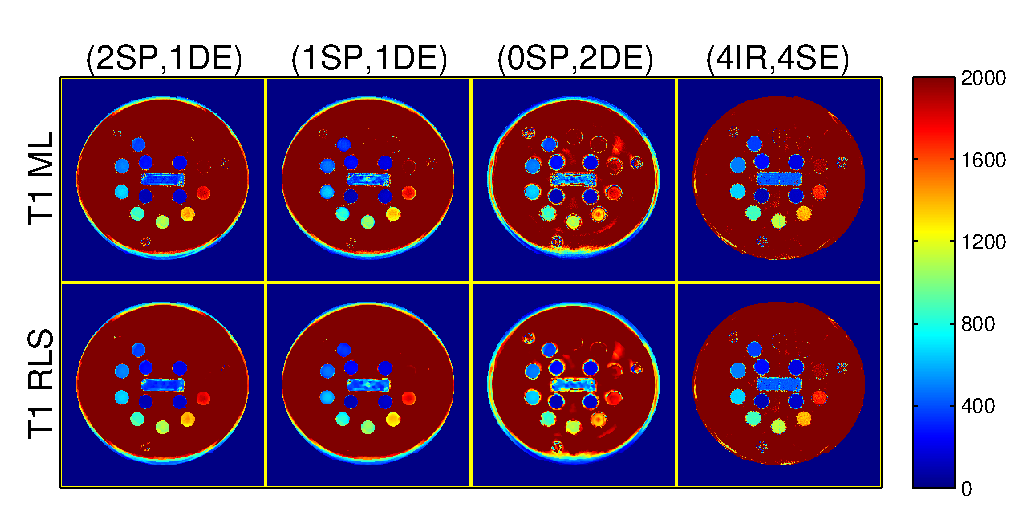
\includegraphics [width=15.4cm] {2016-06-20,hpd,t1,jet.eps}
		\label{fig:hpd,t1,jet}
	}
	\vspace{0cm}
	\subfigure{
		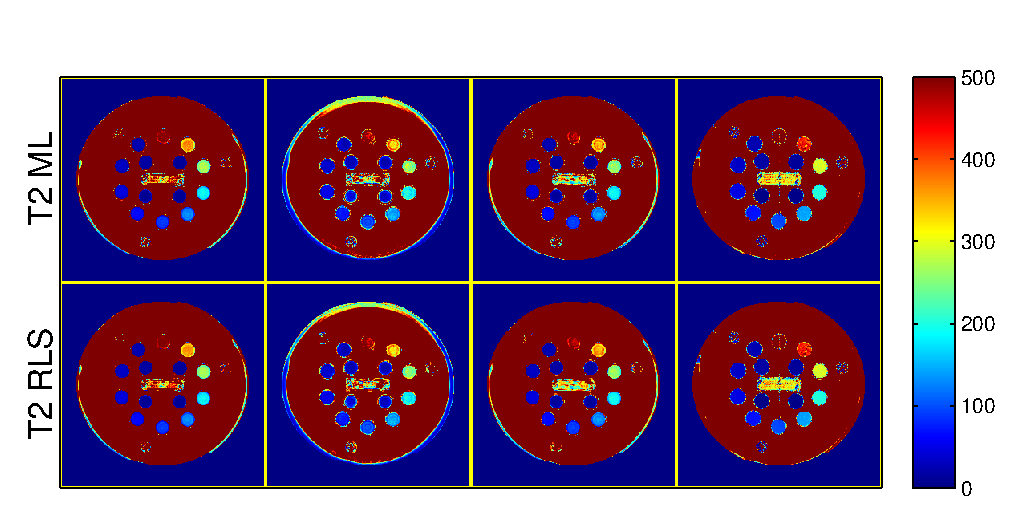
\includegraphics [width=15.2cm, trim=0 0 0 25, clip] {2016-06-20,hpd,t2,jet.eps}
		\label{fig:hpd,t2,jet}
	}
	\caption{
		Colorized $\bmTo$ and $\bmTt$ ML and RL estimates 
		from an HPD\regis quantitative phantom.
		Columns correspond to scan profiles consisting of 
		(2 SPGR, 1 DESS), (1 SPGR, 1 DESS), (0 SPGR, 2 DESS),
		and (4 IR, 4 SE) acquisitions. 
		Rows distinguish $\bmTo$ and $\bmTt$ ML and RL estimators. 
		Fig.~\ref{fig:hpd,gray} provides identical grayscale images
		that enumerate vials.
		Colorbar ranges are in milliseconds.
	}
	\label{fig:hpd,jet}
\end{figure*}

% nist t1/t2 maps, gray
\begin{figure*} [!tb]
	\centering
	\subfigure{
		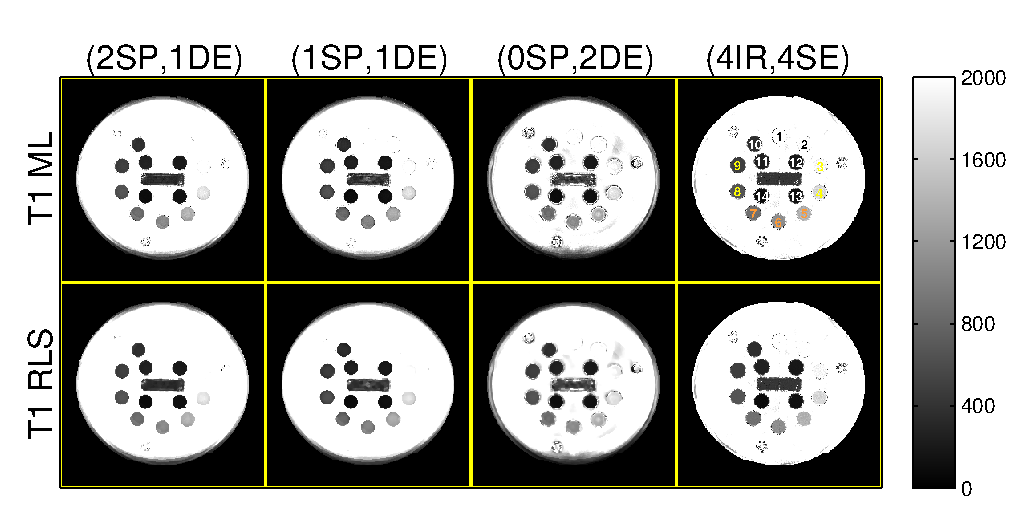
\includegraphics [width=15.4cm] {2016-06-20,hpd,t1,gray.eps}
		\label{fig:hpd,t1,gray}
	}
	\vspace{0cm}
	\subfigure{
		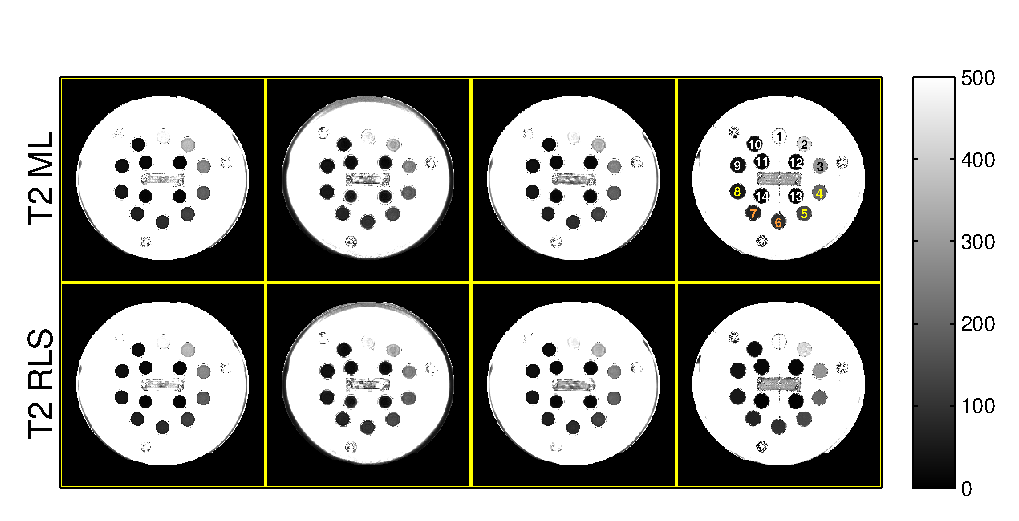
\includegraphics [width=15.2cm, trim=0 0 0 25, clip] {2016-06-20,hpd,t2,gray.eps}
		\label{fig:hpd,t2,gray}
	}
	\caption{
		Grayscale $\bmTo$ and $\bmTt$ ML and RL estimates 
		from an HPD\regis quantitative phantom.
		Columns correspond to scan profiles consisting of 
		(2 SPGR, 1 DESS), (1 SPGR, 1 DESS), (0 SPGR, 2 DESS),
		and (4 IR, 4 SE) acquisitions. 
		Rows distinguish $\bmTo$ and $\bmTt$ ML and RL estimators. 
		Vials are enumerated and color-coded
		to correspond with data points in Fig.~\ref{fig:hpd,ml-rls}.
		Fig.~\ref{fig:hpd,jet} provides identical colorized images.
		Colorbar ranges are in milliseconds.
	}
	\label{fig:hpd,gray}
\end{figure*}

Figs.~\ref{fig:hpd,jet}-\ref{fig:hpd,gray} compare
in color and grayscale  
phantom $\bmTo$ and $\bmTt$ ML and RL estimates 
from optimized scan profiles. 
Vials are enumerated 
in Fig.~\ref{fig:hpd,ml-rls} 
in descending $\To$ and $\Tt$ order. 
Vials corresponding to tight $\setXt$ 
and broad $\setXb$ parameter ranges are highlighted 
with orange and yellow labels, respectively. 
Within these vials of interest, 
parameter maps from different scans appear visually similar.

% outside range of interest, most severe bias in T1 ML (0,2) 
% appears that pure-DESS tends to have significantly greater systematic errors in regions of high T1 
In higher-$\To$ vials (and the surrounding water),
more bias is apparent 
in $\bmToest$ ML and RL estimates 
from the $(0,2)$ scan profile than 
from the $(2,1)$ and $(1,1)$ scan profiles. 
With the signal models used in this study,
the images suggest that scan profiles consisting 
of at least one SPGR scan may offer increased protection 
against $\To$ estimation bias.

% t1/t2 ml/rls hpd accuracy
\begin{figure*} [!tbp]
	\centering
	\subfigure [$\ToML$ Estimates] {
		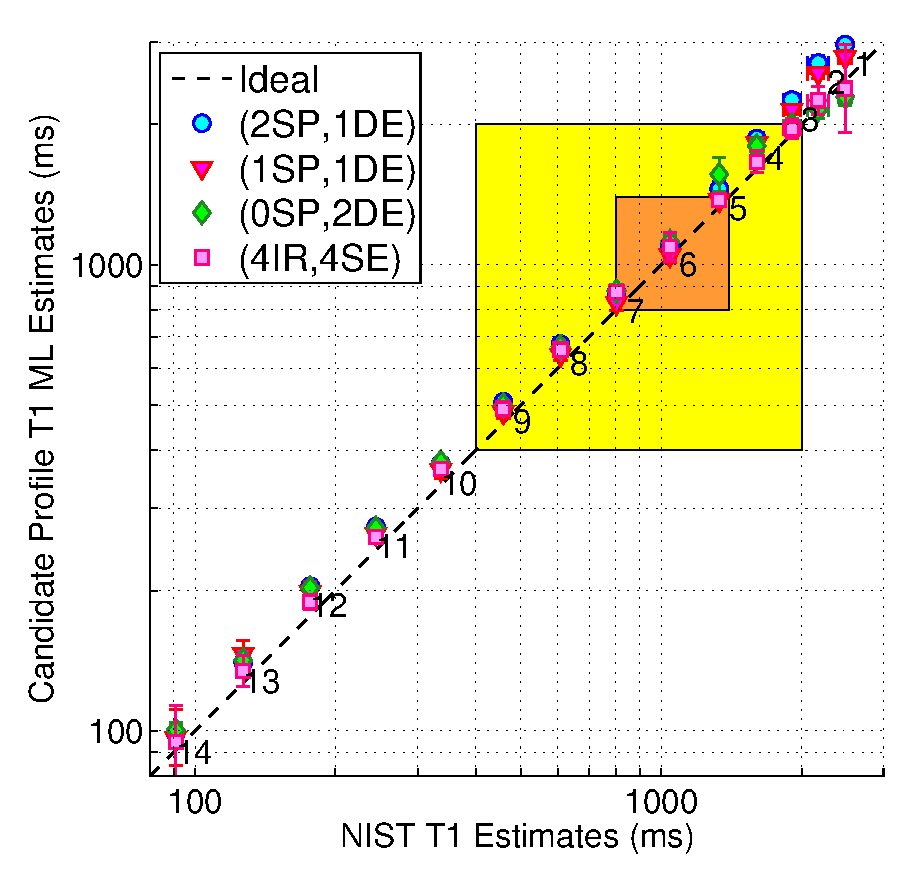
\includegraphics [width = 0.45\textwidth] {2016-06-20,hpd,t1-ml-compare.eps}
		\label{fig:t1,hpd,ml}
	}
	\hspace{0.3cm}
	\subfigure [$\TtML$ Estimates] {
		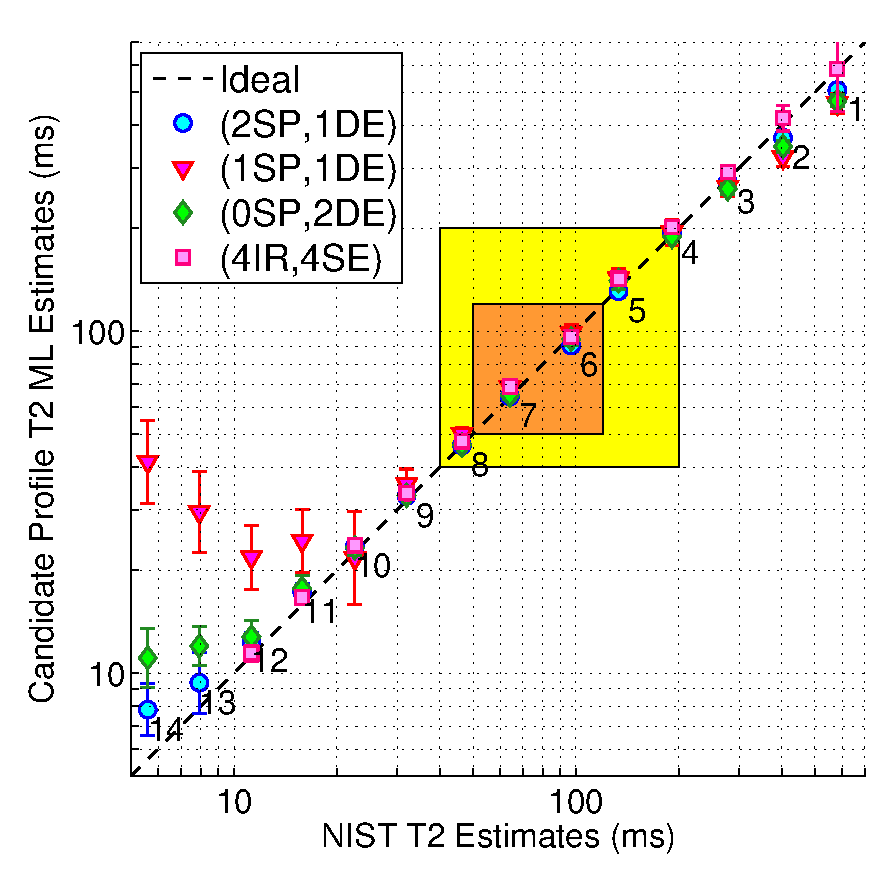
\includegraphics [width = 0.45\textwidth] {2016-06-20,hpd,t2-ml-compare.eps}
		\label{fig:t2,hpd,ml}
	}
	\vspace{-0.3cm}
	\subfigure [$\ToRL$ Estimates] {
		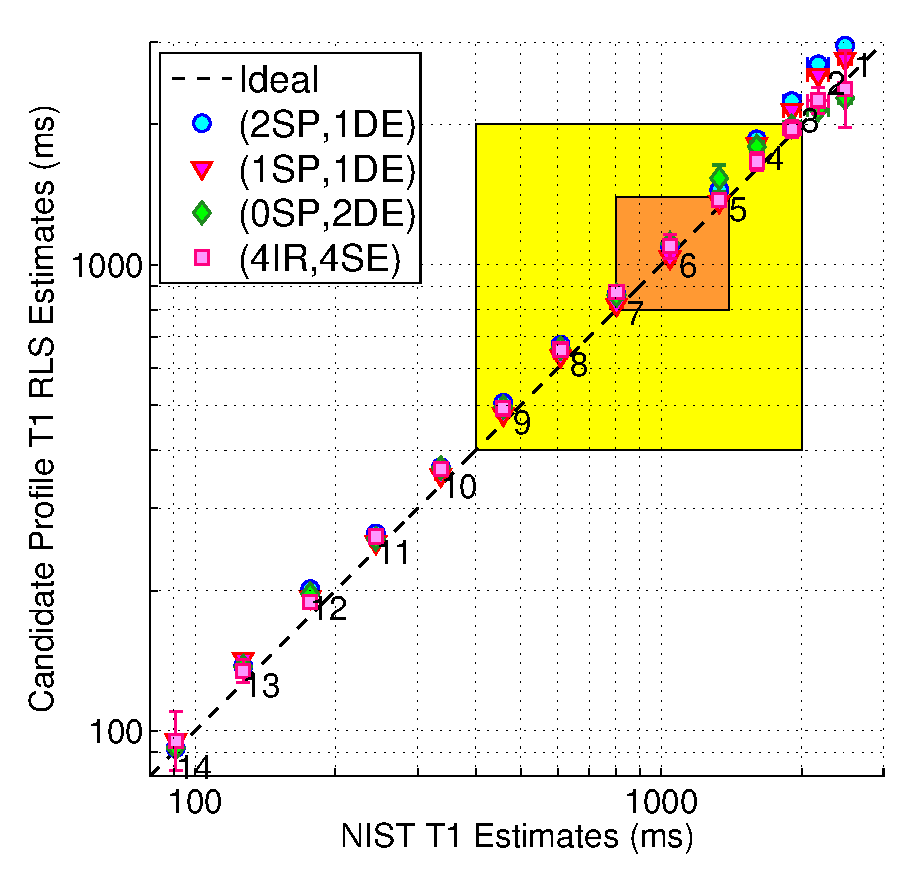
\includegraphics [width = 0.45\textwidth] {2016-06-20,hpd,t1-rls-compare.eps}
		\label{fig:t1,hpd,rls}
	}
	\hspace{0.3cm}
	\subfigure [$\TtRL$ Estimates] {
		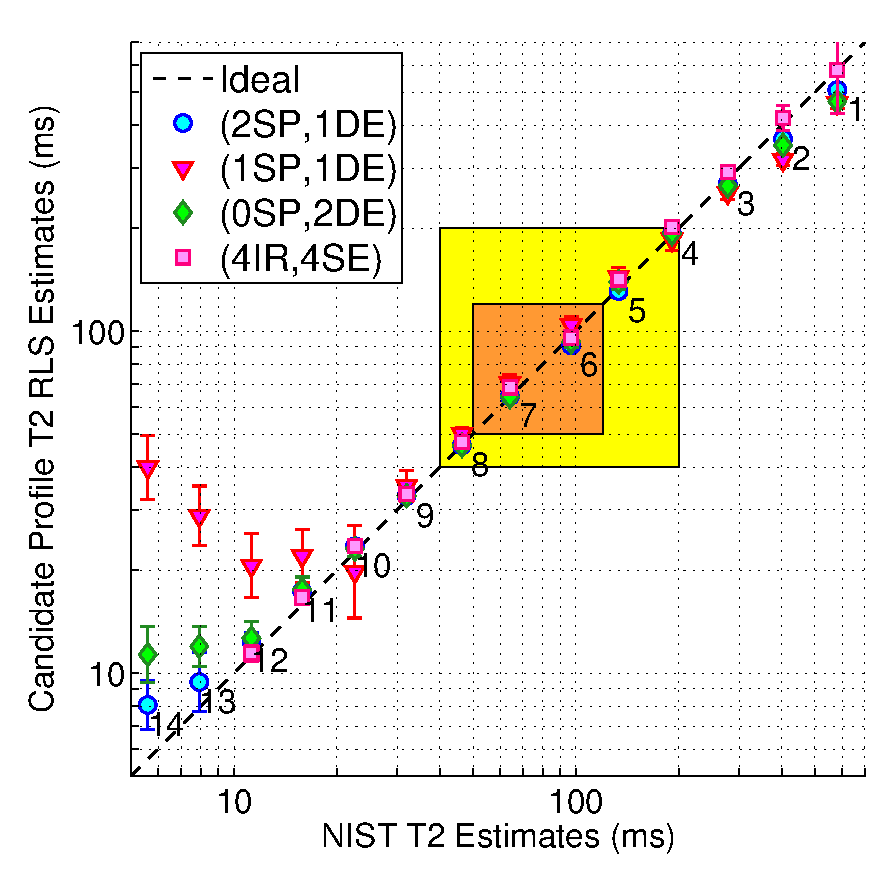
\includegraphics [width = 0.45\textwidth] {2016-06-20,hpd,t2-rls-compare.eps}
		\label{fig:t2,hpd,rls}
	}
	\caption{
		Phantom within-ROI sample statistics 
		of $\bmTo$ and $\bmTt$ ML and RL estimates 
		from optimized SPGR/DESS and reference IR/SE scan profiles, 
		versus NIST NMR measurements \cite{keenan:16:msm}.
		Markers and error bars indicate 
		ROI sample means and ROI sample standard deviations 
		within the 14 labeled and color-coded vials 
		in Fig.~\ref{fig:hpd,gray}.
		Tight $\setXt$ and broad $\setXb$ latent parameter ranges are highlighted 
		in orange and yellow, respectively.
		Table~\ref{table:hpd,accuracy} replicates sample statistics 
		within Vials 5-8.
		Our MR measurements are at 293K 
		and NIST NMR measurements are at 293.00K.
		Within the designed parameter ranges, 
		estimates from different acquisitions 
		are in reasonable agreement with NIST measurements.
	}
	\label{fig:hpd,ml-rls}
\end{figure*}

% t1/t2 ml/rls hpd accuracy-table
\begin{table*} [t]
	\centering
	\begin{tabu} {c || r r r | r || r}
		\hline \hline
		 			& (2SP,1DE)			& (1SP,1DE) 		& (0SP,2DE)			& (4IR,4SE)			& NIST NMR\\
		\hline
		V5 $\ToML$ 	& $1450 \pm 50.$	& $1380 \pm 41$ 	& $1600 \pm 130$	& $1380 \pm 44$		& $1332 \pm 0.8$ \\
		V5 $\ToRL$	& $1450 \pm 26$ 	& $1370 \pm 16$		& $1540 \pm 98$ 	& $1380 \pm 37$		& \\
		\hline
		V6 $\ToML$ 	& $1100 \pm 30.$	& $1050 \pm 39$		& $1120 \pm 39$ 	& $1100 \pm 74$ 	& $1044 \pm 3.2$ \\
		V6 $\ToRL$ 	& $1100 \pm 15$ 	& $1040 \pm 14$ 	& $1110 \pm 16$ 	& $1100 \pm 64$ 	& \\
		\hline
		V7 $\ToML$ 	& $870 \pm 22$ 		& $830 \pm 29$ 		& $880 \pm 29$		& $870 \pm 25$		& $801.7 \pm 1.70$ \\
		V7 $\ToRL$ 	& $865 \pm 7.1$ 	& $820 \pm 11$		& $860 \pm 18$		& $870 \pm 21$		& \\
		\hline
		V8 $\ToML$ 	& $680 \pm 12$ 		& $640 \pm 18$		& $670 \pm 12$ 		& $658 \pm 8.8$ 	& $608.6 \pm 1.03$ \\
		V8 $\ToRL$ 	& $674 \pm 7.6$		& $637 \pm 7.4$ 	& $662 \pm 6.6$		& $658 \pm 7.1$		& \\
		\hline \hline
		V5 $\TtML$ 	& $131 \pm 5.5$		& $140 \pm 10.$		& $141 \pm 8.4$		& $143 \pm 4.9$		& $133.27 \pm 0.073$ \\
		V5 $\TtRL$ 	& $131 \pm 5.2$ 	& $145 \pm 9.1$		& $139 \pm 7.1$		& $142 \pm 4.8$ 	& \\
		\hline
		V6 $\TtML$	& $91 \pm 3.5$ 		& $99 \pm 6.0$ 		& $95 \pm 4.2$ 		& $96 \pm 2.7$ 		& $96.89 \pm 0.049$ \\
		V6 $\TtRL$ 	& $91 \pm 3.4$ 		& $104 \pm 6.2$		& $93 \pm 3.7$ 		& $96 \pm 2.6$		& \\
		\hline
		V7 $\TtML$ 	& $64 \pm 2.2$		& $69 \pm 3.9$		& $65 \pm 2.1$ 		& $69 \pm 1.2$ 		& $64.07 \pm 0.034$ \\
		V7 $\TtRL$ 	& $65 \pm 2.1$ 		& $71 \pm 4.3$		& $64 \pm 1.9$ 		& $69 \pm 1.2$ 		& \\
		\hline
		V8 $\TtML$	& $46 \pm 1.5$ 		& $50. \pm 2.3$ 	& $46 \pm 1.1$		& $47.6 \pm 0.87$ 	& $46.42 \pm 0.014$ \\
		V8 $\TtRL$	& $46 \pm 1.5$ 		& $50. \pm 2.3$ 	& $46 \pm 1.0$ 		& $47.5 \pm 0.85$ 	& \\	
		\hline \hline	 
	\end{tabu}
	\caption{
		Phantom within-ROI sample means $\pm$ sample standard deviations 
		of $\mathbf{T}_1$ and $\mathbf{T}_2$ estimates 
		from optimized SPGR/DESS and reference IR/SE scan profiles, 
		versus NIST NMR measurements (\emph{cf.} slide 22 
		of e-poster corresponding to \cite{keenan:16:msm}).
		For sake of brevity, 
		sample statistics corresponding only to phantom vials 
		within (or nearly within) tight design range $\setXt$ 
		(color-coded orange in Fig.~\ref{fig:hpd,gray}) are reported. 
		Fig.~\ref{fig:hpd,ml-rls} plots sample statistics for all vials.
		`V\#' abbreviates vial numbers. 
		All values are reported in milliseconds.
	}
	\label{table:hpd,accuracy}
\end{table*}

Fig.~\ref{fig:hpd,ml-rls} plots 
sample means and sample standard deviations 
computed within circular ROIs 
of phantom $\bmTo$ and $\bmTt$ ML and RL estimates.
The highlighted orange and yellow parameter spaces 
correspond to design ranges $\setXt$ and $\setXb$.
$\bmTo$ estimates from both 
the candidate $(2,1)$, $(1,1)$, and $(0,2)$ (SPGR, DESS) 
and reference $(4,4)$ (IR, SE) profiles 
are in reasonable agreement 
with NIST estimates \cite{keenan:16:msm} 
across the vial range.
$\bmTt$ estimates from all profiles are also 
in good agreement with NIST 
for vials within $\setXb$.
SPGR/DESS profiles likely underestimate large $\Tt$ values ($\ge$200ms) 
due to greater influence of diffusion in DESS 
\cite{carney:91:asa, wu:90:eod, kaiser:74:daf},
(studied further in Appendix~\ref{a,dess-diff}).
SPGR/DESS profiles possibly overestimate 
and the IR/SE profile likely underestimates 
short ($\le$30ms) and very short ($\le$15ms) $\Tt$ values, 
respectively, 
due to poorly conditioned estimation. 
Table~\ref{table:hpd,accuracy} replicates sample statistics 
in Fig.~\ref{fig:hpd,ml-rls} for vials 5-8.
Compared to ML initializations, 
(weakly) regularized estimates reduce error bars 
without introducing substantial additional bias.

%%%%%%%%%%%%%%%%%%%%%%%%%%%%%%%%%%%%%%%%%%%%%%%%%%%	
\subsubsection{Across-Repetition Statistics} 
\label{sss,scn-dsgn,exp,phant,rep}

\begin{table*} [!tb]
	\centering
	\begin{tabu} {c | r r r}
		\hline \hline
		 								& (2SP,1DE)				& (1SP,1DE) 			& (0SP,2DE)	\\
		\hline
		V5 $\sigToML$ 	& $50 \pm 12$			& $40 \pm 10.$    & $39 \pm 9.4$ \\	
		V6 $\sigToML$ 	& $70 \pm 18$ 		& $60 \pm 15$ 		& $70 \pm 16$ \\
		V7 $\sigToML$ 	& $60 \pm 13$ 		& $50 \pm 13$ 		& $50 \pm 13$ \\
		V8 $\sigToML$ 	& $23 \pm 5.4$ 		& $20. \pm 4.7$		& $18 \pm 4.3$ \\
		\hline \hline
		V5 $\sigTtML$ 	& $2.6 \pm 0.63$	& $6 \pm 1.4$			& $3.5 \pm 0.84$ \\
		V6 $\sigTtML$		& $1.9 \pm 0.46$ 	& $5 \pm 1.1$			& $2.3 \pm 0.54$ \\
		V7 $\sigTtML$ 	& $1.4 \pm 0.34$	& $3.4 \pm 0.80$ 	& $1.5 \pm 0.35$ \\
		V8 $\sigTtML$ 	& $1.1 \pm 0.26$	& $3.5 \pm 0.84$ 	& $1.4 \pm 0.33$ \\
		\hline \hline
	\end{tabu}
	\caption{
		Phantom pooled sample standard deviations 
		$\pm$ pooled standard errors of sample standard deviations, 
		from optimized SPGR/DESS scan profiles.
		Each entry is a measure of uncertainty 
		of a typical voxel's $\To$ or $\Tt$ ML estimate,
		estimated over 10 repeated acquisitions.
		For sake of brevity, 
		sample statistics corresponding only 
		to phantom vials within 
		(or nearly within) 
		tight design range $\setXt$
		(color-coded orange in Fig.~\ref{fig:hpd,gray}) 
		are reported. 	
		`V\#' abbreviates vial numbers. 
		All values are reported in milliseconds.
	}
	\label{table:hpd,sample-std-dev}
\end{table*}

In a second study, 
we repeat the $(2,1)$, $(1,1)$, and $(0,2)$ scan profiles 
10 times each 
and separately compute $\bmTo$ and $\bmTt$ ML estimates
for each repetition of each scan profile. 
We then estimate the standard deviation across repetitions 
on a per-voxel basis, 
to produce sample standard deviation maps 
for each profile.
Each ROI voxel of the sample standard deviation map 
is a better estimate 
of the \emph{population standard deviation} 
(which the CRB characterizes) 
than the ROI sample standard deviation 
from a single repetition, 
because the latter estimate is contaminated 
with slight spatial variation 
of voxel population means 
(due to imaging non-idealities 
such as Gibbs ringing 
due to $\mathbf{k}$-space truncation).
	
Table~\ref{table:hpd,sample-std-dev} reports 
pooled sample standard deviations 
and pooled standard errors of the sample standard deviations 
(computed via expressions in \cite{ahn:03:seo}) 
for phantom vials within (or nearly within) 
tight design range $\setXt$ 
(marked orange in Fig.~\ref{fig:hpd,gray}).
Due to error propagation from coil combination 
and $\bmstx$ estimation, 
pooled ML sample standard deviations 
cannot be compared \emph{in magnitude} 
to worst-case predicted standard deviations 
(Table~\ref{table:profile}); 
however, \emph{trends} 
of empirical and theoretical standard deviations 
are overall similar.
In particular, 
the optimized $(0,2)$ DESS-only scan profile 
affords $\To$ ML estimation precision 
(in vials whose $\To,\Tt$ is similar to that of WM/GM) 
comparable to optimized $(2,1)$ and $(1,1)$ 
mixed (SPGR, DESS) profiles. 
Also in agreement with predictions, 
the optimized $(2,1)$ and $(0,2)$ profiles 
afford greater $\Tt$ ML estimation precision 
than the optimized $(1,1)$ profile.

%%%%%%%%%%%%%%%%%%%%%%%%%%%%%%%%%%%%%%%%%%%%%%%%%%%
\subsection{\textit{In~Vivo} Experiments}
\label{ss,scn-dsgn,exp,invivo}

In a single long study of a healthy volunteer, 
we acquire the same optimized scan profiles 
containing $(2,1)$, $(1,1)$, and $(0,2)$ SPGR/DESS scans 
(\emph{cf.} Table~\ref{table:profile}), 
as well as the reference profile 
containing $(4,4)$ IR/SE scans.
We obtain axial slices 
from a 32-channel Nova Medical\regis receive head array.
To address bulk motion between acquisitions 
and to compare within-ROI statistics, 
we rigidly register
\footnote{For each coil-combined dataset, 
we compute a separate 2D rigid transformation 
(with respect to the $\TI = 50$ms IR dataset) 
via the MATLAB\regis function \texttt{imregtform} 
and then apply the transformation via \texttt{imwarp}.
We choose to use rigid transformations 
instead of affine distortions to avoid scaling; 
however in doing so we sacrifice compensating 
for small through-plane rotations. 
We do not find registration 
to substantially change subsequently estimated relaxation maps; 
however, this extra step substantially improves alignment 
of (especially cortical GM) ROIs 
in $\To$ and $\Tt$ estimates from different scan profiles.
} 
each coil-combined image to an IR image
prior to parameter mapping.
All acquisition and reconstruction details 
are otherwise the same as in phantom experiments
(\emph{cf.} Section~\ref{sss,scn-dsgn,exp,phant,roi}). 
For all SS scan profiles tested, 
ML and RL reconstructions 
of brain datasets require less than 3m30s and 9s, respectively.

% brain t1/t2 maps, jet
\begin{figure*} [!tbp]
	\centering
	\subfigure{
		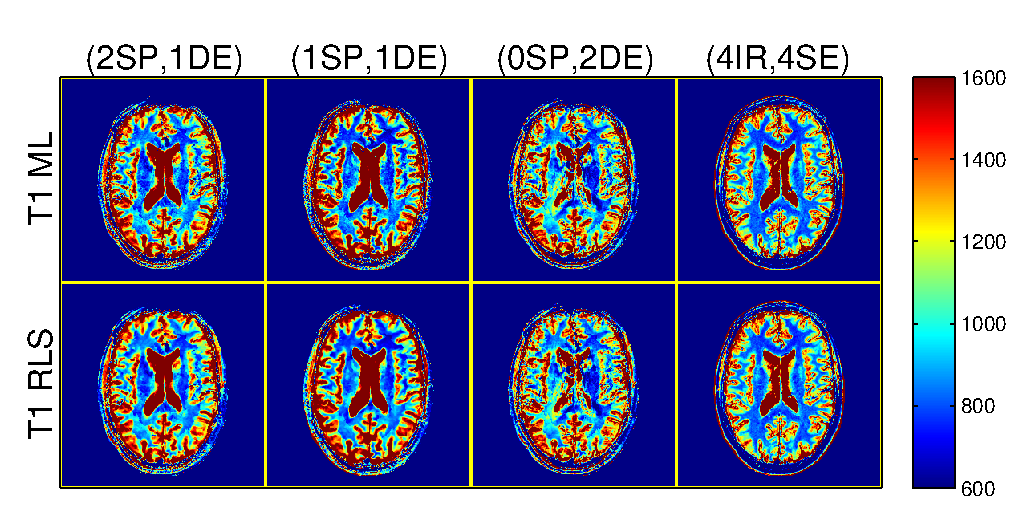
\includegraphics [width=15.4cm] {2016-05-31,brain,t1,jet.eps}
		\label{fig:brain,t1,jet}
	}
	\vspace{0cm}
	\subfigure{
		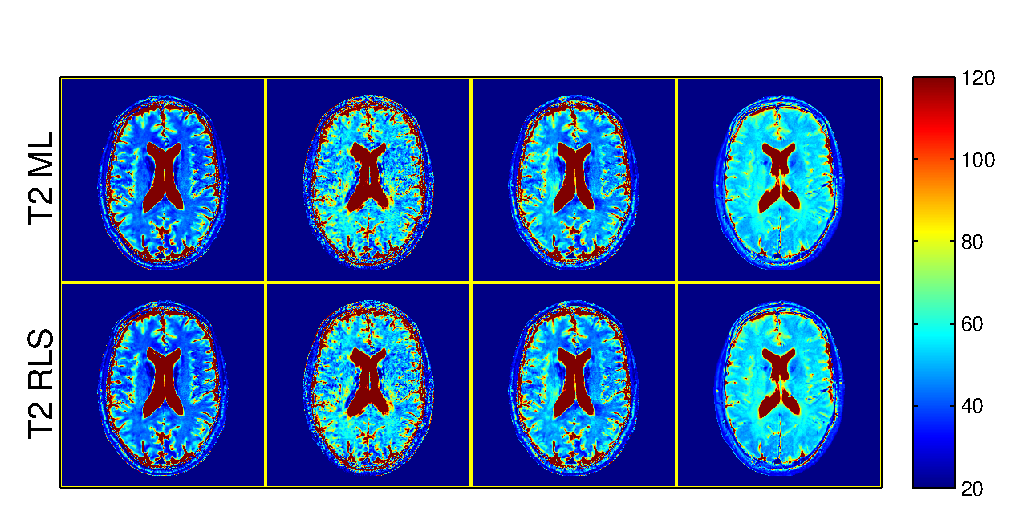
\includegraphics [width=15.2cm, trim=0 0 0 25, clip] {2016-05-31,brain,t2,jet.eps}
		\label{fig:brain,t2,jet}
	}
	\caption{
		Colorized $\bmTo$ and $\bmTt$ ML and RL estimates 
		from the brain of a healthy volunteer.
		Columns correspond to profiles consisting 
		of (2~SPGR,~1~DESS), (1~SPGR,~1~DESS), (0~SPGR,~2~DESS), 
		and (4~IR,~4~SE) acquisitions.  
		Rows distinguish $\bmTo$ and $\bmTt$ ML and RL estimators.
		Table~\ref{table:brain} presents corresponding WM/GM 
		within-ROI sample statistics.
		Colorbar ranges are in milliseconds.
	}
	\label{fig:brain,jet}
\end{figure*}

Fig.~\ref{fig:brain,jet} compares 
brain $\bmTo$ and $\bmTt$ ML and RL estimates 
from optimized scan profiles.
Though in-plane motion is largely compensated via registration, 
through-plane motion and non-bulk motion likely persist, 
and will influence ROI statistics.
Due to motion (and scan duration) considerations,
we examine within-ROI statistics from a single repetition 
as in Section~\ref{sss,scn-dsgn,exp,phant,roi}, 
and do not attempt across-repetition statistics 
as in Section~\ref{sss,scn-dsgn,exp,phant,rep}.
	
Visually, $\bmToest$ maps from steady-state profiles 
exhibit similar levels of contrast 
in WM/GM regions well away 
from cerebrospinal fluid (CSF) as that seen 
in the reference $\bmToest$ estimate.
Since we did not optimize any scan profiles 
for estimation in high-$\To$ regions, 
it is expected that greater differences may emerge 
in voxels containing or nearby CSF. 
In particular, 
$\bmTo$ is significantly underestimated 
within and near CSF by the $(0,2)$ DESS-only profile. 
This suggests that with the signal models used in this work, 
including at least one SPGR scan in an optimized profile 
may offer greater protection 
against estimation bias in high-$\To$ regions.

% t1/t2 ml brain summary table
\begin{table*} [tb]
	\centering
	\small
	\begin{minipage}{0.18\textwidth}
		\includegraphics [width=2.8cm] {2016-05-31,brain,roi,gray.eps}
		\label{fig:brain,roi,gray}
	\end{minipage}
	\begin{minipage}{0.8\textwidth}
		\begin{tabu} {c | c | r r r | r}
			\hline \hline
				& ROI			& (2SP,1DE)				& (1SP,1DE) 			& (0SP,2DE)				& (4IR,4SE) \\
			\hline
			\multirow{5}{*}{$\ToML$} 	
			& \AR WM	& $840 \pm 32$		& $770 \pm 31$ 		& $840 \pm 43$ 		& $780 \pm 22$ \\
			& \AL WM 	& $740 \pm 61$ 		& $660 \pm 45$ 		& $740 \pm 55$ 		& $760 \pm 24$ \\
			& \PR WM 	& $890 \pm 88$ 		& $860 \pm 72$ 		& $960 \pm 84$ 		& $810 \pm 26$ \\
			& \PL WM 	& $860 \pm 70.$ 	& $850 \pm 61$ 		& $880 \pm 79$ 		& $820 \pm 37$ \\
			& \A GM 	& $1200 \pm 210$	& $1200 \pm 230$ 	& $1300 \pm 230$	& $1300 \pm 180$ \\
			\hline
			\multirow{5}{*}{$\ToRL$} 	
			& \AR WM	& $840 \pm 24$		& $770 \pm 20.$		& $840 \pm 43$ 		& $780 \pm 20.$ \\
			& \AL WM 	& $740 \pm 51$ 		& $670 \pm 37$ 		& $740 \pm 54$ 		& $760 \pm 23$ \\
			& \PR WM 	& $890 \pm 79$ 		& $860 \pm 61$ 		& $960 \pm 82$ 		& $810 \pm 24$ \\
			& \PL WM 	& $870 \pm 62$ 		& $850 \pm 50.$		& $880 \pm 78$ 		& $820 \pm 35$ \\
			& \A GM 	& $1200 \pm 200$	& $1200 \pm 220$ 	& $1300 \pm 230$	& $1300 \pm 180$ \\
			\hline \hline
			\multirow{5}{*}{$\TtML$} 	
			& \AR WM 	& $40. \pm 1.3$ 	& $54 \pm 3.8$ 		& $46 \pm 1.5$		& $55 \pm 1.9$ \\
			& \AL WM 	& $40. \pm 1.7$		& $50. \pm 4.5$		& $44 \pm 1.7$ 		& $53 \pm 1.8$ \\
			& \PR WM  & $43 \pm 2.7$ 		& $60. \pm 6.9$ 	& $51 \pm 3.6$ 		& $59 \pm 2.1$ \\
			& \PL WM 	& $43 \pm 1.8$		& $57 \pm 4.9$ 		& $49 \pm 2.5$ 		& $57 \pm 1.8$ \\
			& \A GM 	& $50 \pm 12$ 		& $60 \pm 15$ 		& $60 \pm 11$ 		& $59 \pm 6.0$ \\
			\hline
			\multirow{5}{*}{$\TtRL$} 	
			& \AR WM  & $40. \pm 1.3$ 	& $54 \pm 3.4$ 		& $46 \pm 1.5$		& $55 \pm 1.9$ \\
			& \AL WM 	& $40. \pm 1.7$		& $50. \pm 4.4$		& $43 \pm 1.7$ 		& $53 \pm 1.8$ \\
			& \PR WM  & $43 \pm 2.8$ 		& $60. \pm 6.7$ 	& $51 \pm 3.7$ 		& $58 \pm 2.3$ \\
			& \PL WM 	& $43 \pm 1.7$		& $57 \pm 4.7$ 		& $49 \pm 2.5$ 		& $57 \pm 1.8$ \\
			& \A GM 	& $50 \pm 12$ 		& $60 \pm 15$ 		& $60 \pm 11$ 		& $59 \pm 6.4$ \\
			\hline \hline
		\end{tabu}
	\end{minipage}
	\vspace{1mm}
	\caption{
		\emph{Left}:
		WM/GM ROIs,
		overlaid on a representative anatomical
		(coil-combined, IR) image.
		Separate WM ROIs are distinguished
		by anterior-right (\AR),
		anterior-left (\AL),
		posterior-right (\PR), and
		posterior-left (\PL) directions.
		Four small anterior (\A) cortical GM polygons
		are pooled into a single ROI.
		\emph{Right}:
		Within-ROI sample means $\pm$ 
		within-ROI sample standard deviations 
		of $\bmTo$ and $\bmTt$ ML and RL estimates 
		from the brain of a healthy volunteer
		(Fig.~\ref{fig:brain,jet} presents corresponding images).
		Sample statistics are computed 
		within ROIs indicated in the anatomical image.  
		All values are reported in milliseconds.
	}
	\label{table:brain}
\end{table*} 

Table~\ref{table:brain} summarizes 
within-ROI sample means and sample standard deviations 
computed\footnote{We have taken effort 
to select ROIs that reflect expected anatomy 
in all coil-combined and registered images, 
including adjacent slices in images from 3D acquisitions. 
However, we acknowledge the possibility 
of some contamination across tissue boundaries, 
especially WM and/or CSF contamination into cortical GM.
}
over four separate WM ROIs containing 96, 69, 224, and 148 voxels 
and one pooled cortical GM ROI containing 156 voxels.	
Within-ROI $\bmToest$ sample standard deviations are comparable 
across SS profiles.
In agreement with Table~\ref{table:profile}, 
$\bmTt$ estimates from the optimized $(1,1)$ scan profile 
exhibit higher within-ROI sample variation 
than corresponding $(2,1)$ and $(0,2)$ $\bmTtest$ maps.
Compared to ML counterparts,
RL estimates generally reduce within-ROI sample variation
and do not significantly change within-ROI sample means.

In most cases, $\bmToest$ within-ROI sample means 
from optimized SPGR/DESS scan profiles 
do not deviate substantially from each other 
or from reference IR/SE measurements.
Two notable exceptions are $\ToML$ 
in anterior left and posterior right WM 
from $(1,1)$ and $(0,2)$ profiles: 
these estimates are significantly lower and higher 
than analogous estimates from other profiles, respectively.
Results thus suggest that the optimized $(2,1)$ scan profile 
yields WM $\ToML$ estimates 
that are more consistently similar to IR WM $\ToML$ estimates 
than other optimized SPGR/DESS profiles.

Systematic differences in $\bmTtest$ sample means 
are evident across scan profiles, 
particularly within WM ROIs.
Curiously, the $(1,1)$ profile agrees most consistently 
(in WM/GM $\TtML$ within-ROI sample mean) 
with reference estimates, 
though with relatively high sample variation.
The $(2,1)$ and $(0,2)$ SPGR/DESS profiles 
produce consistently lower WM $\TtML$ 
than the reference IR/SE profile, 
though the $(0,2)$ profile is in reasonable agreement 
with other steady-state estimates \cite{heule:14:tes-nib}.
These discrepancies may due to differences 
in sensitivity to multi-compartmental relaxation \cite{mackay:94:ivv}.
Specifically, different signal models 
with different scan parameter choices 
might be more or less sensitive 
to the model mismatch incurred 
by neglecting to distinguish 
the multiple $\Tt$ components within each voxel.
Chapter~\ref{c,mwf} studies multi-compartmental relaxation 
in much greater detail.

%%%%%%%%%%%%%%%%%%%%%%%%%%%%%%%%%%%%%%%%%%%%%%%%%%%
\section{Discussion and Future Work}
\label{s,scn-dsgn,disc}
%%%%%%%%%%%%%%%%%%%%%%%%%%%%%%%%%%%%%%%%%%%%%%%%%%%

Phantom experiments show 
that optimized scan profiles consisting 
of $(2,1)$, $(1,1)$, and $(0,2)$ (SPGR, DESS) scans 
yield accurate WM/GM $\To,\Tt$ estimates, 
and that empirical precision trends across profiles agree reasonably 
with CRB-based predictions.
However, \emph{in vivo} experiments reveal 
that even with scan optimization, 
it may be challenging to achieve clinically viable levels 
of precision from the aforementioned SS profiles, at least at 3T. 
At the expense of greater scan time, 
it is of course possible that optimized profiles 
containing greater numbers of SPGR, DESS, and/or other SS scans 
can provide clinically acceptable precision levels.
For these and other more complicated scan profiles, 
estimator dependence on scan parameters becomes even less intuitive, 
increasing the need for scan design.

The proposed scan design framework addresses spatial variation 
in object parameters through a min-max design criterion.
The min-max criterion guarantees an upper bound 
on a weighted sum of variances 
and assumes no prior knowledge of distributions.
However, in general it is non-differentiable 
in $\bmP$, precluding gradient-based optimization. 	
Furthermore, it is conservative by nature, 
and often selects scan parameters based 
on corner cases of the object parameter space.
To reduce the influence of corner cases, 
it may be desirable to instead construct a cost function 
related to the coefficient of variation 
as in \cite{jones:96:oss, zhang:98:dos, imran:99:tpm, deoni:04:doo}, 
perhaps by setting parameter weights $\bmW^{-1} \gets \diag{\bmx}$ 
for $\bmx \neq 0$ in \eqref{eq:scn-dsgn,cost}.
	
As a less conservative alternative 
to min-max design, 
other recent works \cite{akcakaya:15:ots, lewis:16:ddo} 
have addressed object parameter spatial variation 
by instead constructing cost functions related 
to the Bayesian CRB \cite{gill:95:aot}, 
which characterizes the expected precision 
with respect to a prior distribution on object parameters.
Bayesian cost functions are usually differentiable and can also, 
with appropriate priors, 
penalize object parameter coefficients of variation 
instead of variances, 
as in \cite{akcakaya:15:ots}.
However, prior distributions are generally unknown, 
and may need to be estimated from data, 
as in \cite{lewis:16:ddo}.

Careful calibration of flip angle scaling $\bmstx$ is essential 
for accurate $\bmTo, \bmTt$ estimation 
from SPGR/DESS scan profiles. 
In this work, we estimate $\bmstx$ 
from \emph{separate} acquisitions 
and adjust nominal flip angles prior to reconstruction, 
but acknowledge that non-idealities 
in those separate acquisitions may themselves 
cause resultant transmit field estimation errors 
to propagate into our $\bmTo,\bmTt$ estimates. 
To reduce error propagation, 
it may be desirable to instead design scan profiles 
to permit \emph{joint} estimation of $\bmstx$, 
in addition to other latent object parameters.
Unfortunately, 
we find that optimizing the $(2,1)$ or $(0,2)$ profile 
to allow for four-parameter 
$\bmx\pr \gets \brac{\To\pr, \Tt\pr, \const{2}\pr, \stx\pr}\tpose$ estimation 
results in unacceptably high amplification 
of the worst-case $\To$ standard deviation. 
(Incidentally however, precise $\bmTt$ ML and RL estimation alone 
from the $(2,1)$ or $(0,2)$ profile 
is possible \cite{nataraj:14:mbe}.) 
It remains an open scan design question 
as to whether time spent collecting Bloch-Siegert data 
for separate $\bmstx$ mapping could instead be better spent 
collecting additional SPGR, DESS, 
and/or other data for joint estimation.

By working with closed-form signal expressions, 
we neglect to model several higher-order effects.
However, it is apparent 
that the nonlinear estimation procedures required 
for many mapping problems can amplify the influence 
of these secondary effects, 
often inducing substantial bias. 
Since the CRB (as described) 
applies only to unbiased estimators, 
it is thus desirable to use signal models 
that are as complete as possible 
for CRB-based scan design.
In theory, scan optimization approach \eqref{eq:scn-dsgn,P-star} 
is even compatible with acquisitions 
where a closed-form model relating data 
to latent and scan parameters is unknown, 
as in \cite{beneliezer:15:raa, ma:13:mrf}. 
In practice, difficulties arise in efficient computation 
of signal gradients required in \eqref{eq:scn-dsgn,fisher},
which may demand more specialized techniques, 
as in \cite{zhao:16:oed}.
Designing scan profiles involving such complex signal models 
would likely necessitate optimization techniques more involved 
than the simple grid searches used in this work.

%%%%%%%%%%%%%%%%%%%%%%%%%%%%%%%%%%%%%%%%%%%%%%%%%%%
\section{Conclusion}
\label{s,scn-dsgn,conc}
%%%%%%%%%%%%%%%%%%%%%%%%%%%%%%%%%%%%%%%%%%%%%%%%%%%

This chapter has introduced 
a CRB-inspired min-max optimization approach 
to guide MR scan design 
for precise parameter estimation. 
As a detailed example, 
we have optimized combinations 
of fast SPGR and DESS scans 
for $\To, \Tt$ relaxometry 
in WM and GM regions of the human brain at 3T. 
Numerical simulations show that at typical noise levels 
and with accurate flip angle prior knowledge, 
WM- and GM-like $\To, \Tt$ ML estimates 
from optimized scans are nearly unbiased,
and so worst-case CRB predictions 
yield reliable bounds on ROI sample variances.
Phantom accuracy experiments show that optimized combinations 
of $(2,1)$, $(1,1)$, or $(0,2)$ (SPGR, DESS) scans 
are in excellent agreement with NIST and IR/SE measurements 
over the designed latent object parameter range of interest.
Phantom precision experiments show 
that these SPGR/DESS combinations exhibit trends 
in pooled sample standard deviations 
that reasonably reflect CRB predictions.

\emph{In vivo} experiments suggest that with optimization, 
the $(0,2)$ profile can yield comparable $\bmToest, \bmTtest$ precision 
to the more conventional $(2,1)$ \cite{nataraj:14:mbe} scan profile 
in well-isolated WM/GM ROIs; 
however, the $(0,2)$ $\bmTo$ estimates are unreliable 
within and near the CSF
and do not agree with IR measurements 
in WM as consistently as the $(2,1)$ profile.
This and other disagreements across profiles \emph{in vivo} 
may be attributable to differences in signal model sensitivities 
to neglected higher-order effects. 
Nevertheless, the example application 
studied in this chapter illustrates 
that scan optimization can enable new parameter mapping techniques 
from established pulse sequences.
